\section{Recommendations for Run 2 b-taggers}

\subsection{High level taggers: DL1 series}

We combine the low level taggers into a high-level one, the DL1r algorithm, combining information from the low-level taggers:
\begin{itemize}%[noitemsep]
	\item The IP2D and IP3D: $\log p_b$
	\item The RNNIP outputs: $p_b$, $p_c$, and $p_l$
	\item The SV1 vertex information (variables in \Tab{\ref{tab:sv1-inputs}})
	\item The JF displaced vertices characteristics, \Tab{\ref{tab:sv1-inputs}}.
\end{itemize} 


The comparisons that we'll show are again

\begin{itemize}
%\itemsep{0em}
	\item Explain architecture, optimization
	\item Explain default values
	\item pre-processing:  mean 0 and standard deviation 1 (except for the binary check variables)
\end{itemize} 

\subsection{Evaluating tagger performance}


\subsection{PFlow optimization}

\textbf{Hybrid sample definition}

In the course of the completion of this thesis, the collaboration switched from using EMTopo jets (which reconstruct a jet from the topo clusters in the calorimeter) to  using PFlow jets which cluster a jet using particle flow candidates that takes into account the better resolution of the tracker for reconstructing lower momentum objects. This improves the jet reconstruction algorithm in two ways. (1) We gain a better reconstruction of the jet \pt resolution (shown by 

\begin{itemize}
	\item Switching from EMTopo to PFlow
	\item Main improvement that we expected for $b$-tagging would be better with the better angular resolution for the jet axis
\end{itemize}

\begin{figure}[htbp]
  \centering
  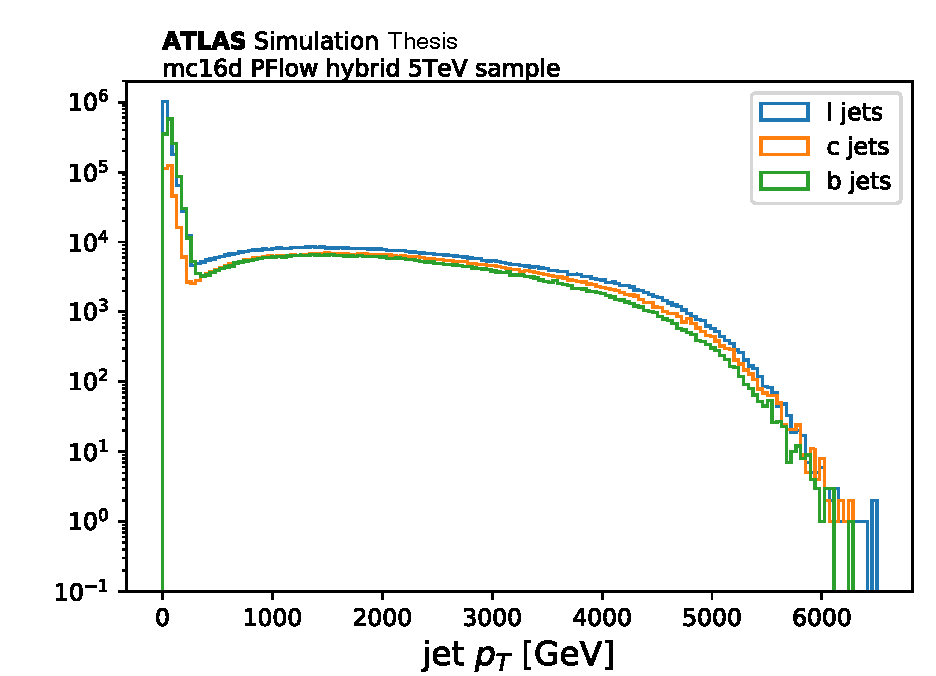
\includegraphics[width=.6\textwidth]{figures/ftag/PFlow trainings/pflow-pt-extended-hybrid}
  \caption{The \pt spectrum for training the Full Run 2 FTAG recommendations.}
  \label{fig:pflow-pt-extended-hybrid}
\end{figure}



\textbf{RNNIP optimization}

An illustration of why the task of \Pqb-tagging becomes harder at high \pt is illustrated in \Fig{\ref{fig:hf-ftag-tracks}}.


\begin{figure}[htbp]
  \centering
  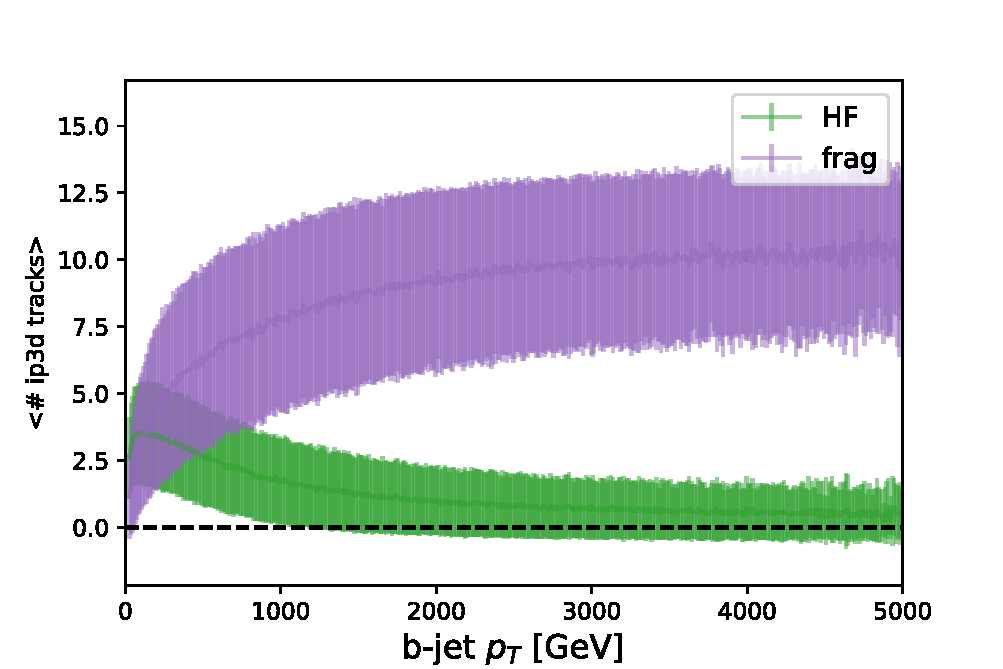
\includegraphics[width=.6\textwidth]{figures/ftag/PFlow trainings/hf-frag-tracks}
  \caption{The evolution of heavy flavor compared to the number of fragmentation tracks that have $\pt > 1~\mathrm{GeV}$, $|d_0| < 1$~mm, $|z_0 \sin \theta < 1.5$~mm, .}
  \label{fig:hf-frag-tracks}
\end{figure}


Our optimization for the RNNIP training for the PFlow tagger uses 400 hidden units in the \ldots LSTM cell.
This is an increase from the 50 hidden units of \cite{ATL-PHYS-PUB-2017-003} since training over the much larger dynamic range needed a more complex architecture.
\textbf{Do I remember what lr I used?}
The training was done with the adam optimizer, using 5 million jets, and 20\% of the dataset was held out as a validation set, and the training was stopped when the validation loss had not improved in the last 20 epochs.


\begin{figure}
\centering
\subfloat[light rejection]{
	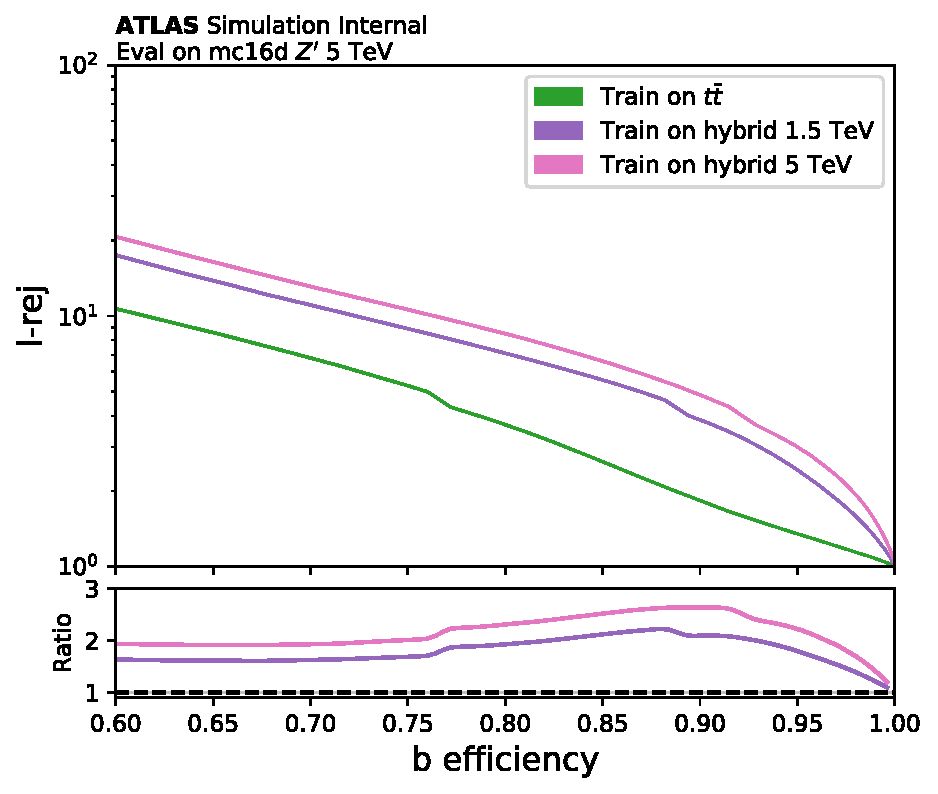
\includegraphics[width=0.45\textwidth]{{figures/ftag/PFlow\ Trainings/Zprime-l-roc}}
	}
\subfloat[\Pqc rejection]{
	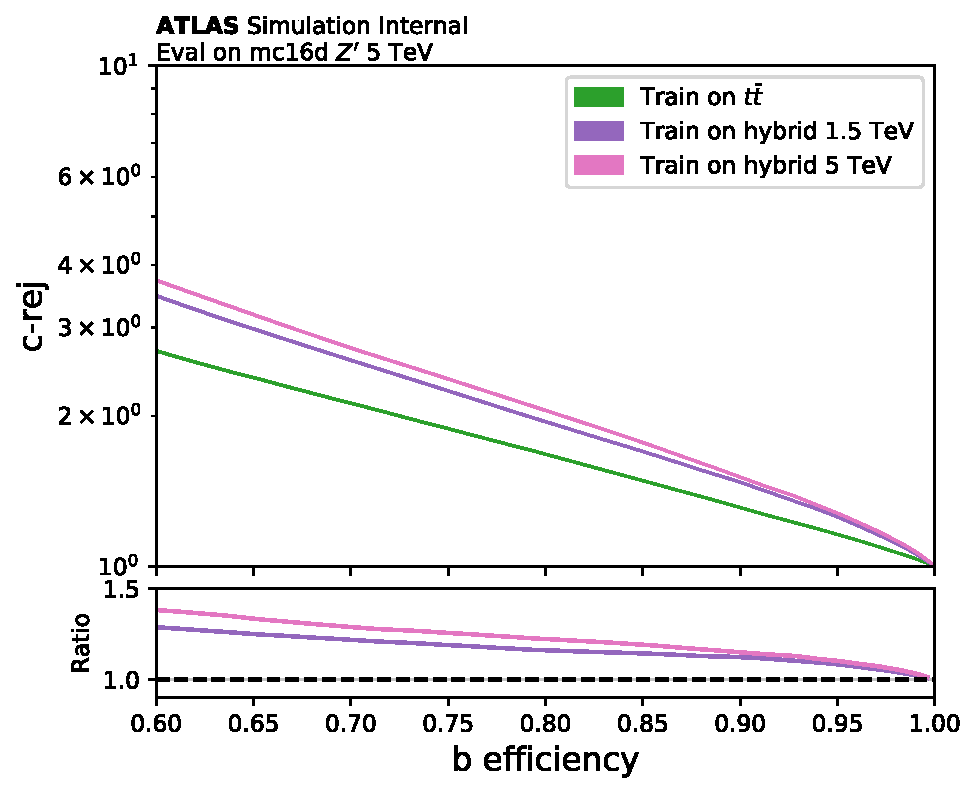
\includegraphics[width=0.45\textwidth]{{figures/ftag/PFlow\ Trainings/Zprime-c-roc}}
	}
\caption{}
\label{fig:Zprime-c-roc}
\end{figure}


\begin{figure}
\centering
\subfloat[light rejection]{
	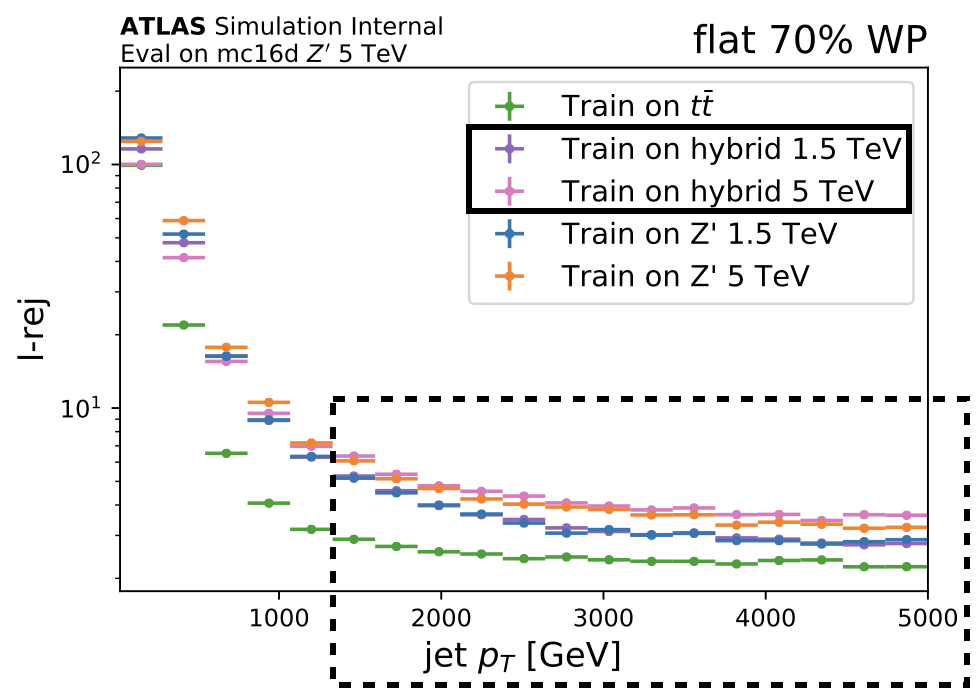
\includegraphics[width=0.45\textwidth]{{figures/ftag/PFlow\ Trainings/Zprime-l-pt}}
	}
\subfloat[\Pqc rejection]{
	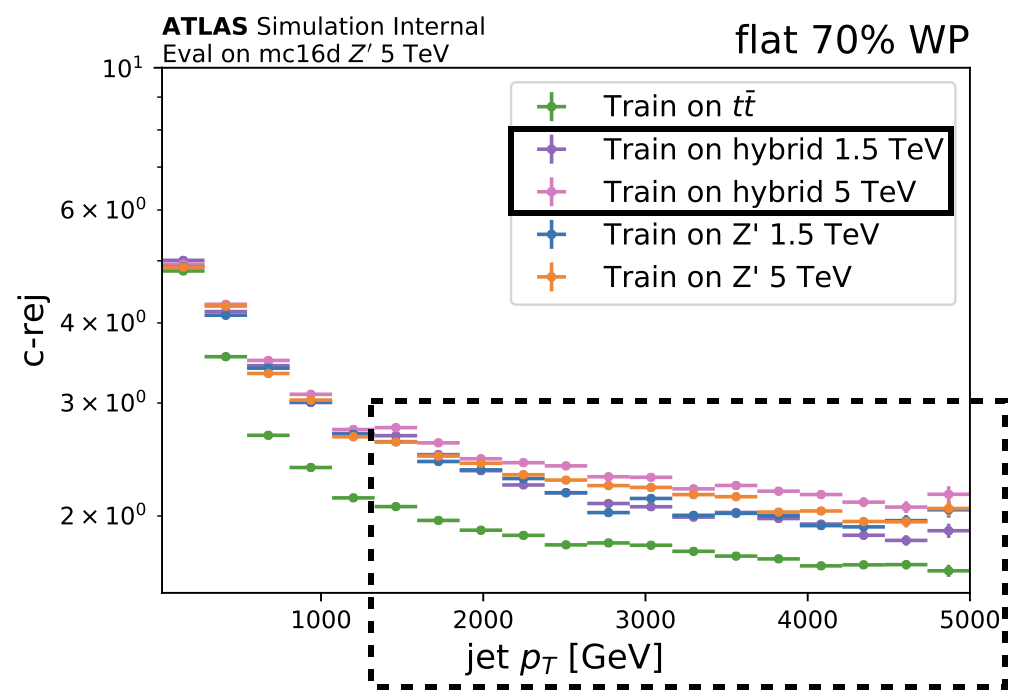
\includegraphics[width=0.45\textwidth]{{figures/ftag/PFlow\ Trainings/Zprime-c-pt}}
	}
\caption{}
\label{fig:Zprime-pt}
\end{figure}



\begin{figure}
\centering
\subfloat[light rejection]{
	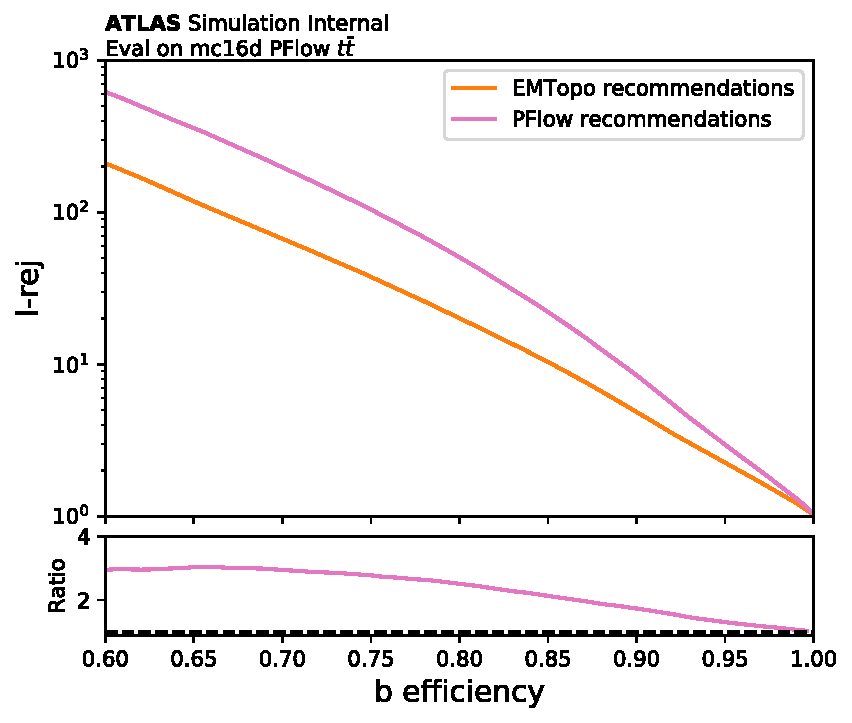
\includegraphics[width=0.45\textwidth]{{figures/ftag/PFlow\ Trainings/topo-vs-pflow-l-rej}}
	}
\subfloat[\Pqc rejection]{
	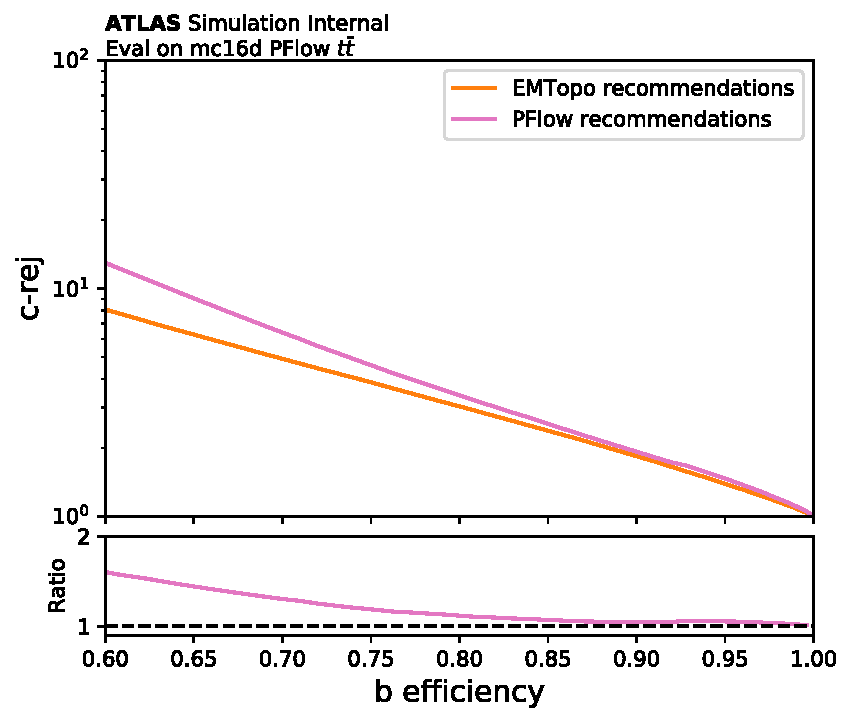
\includegraphics[width=0.45\textwidth]{{figures/ftag/PFlow\ Trainings/topo-vs-pflow-c-rej}}
	}
\caption{}
\label{fig:topo-pflow}
\end{figure}

The EMTopo training recommendation was from the 2017 retraining campaign:

Rafael showed we see retraining gains due to the kinematics changes with hdamp from mc15 -> mc16

Dedicated retraining on new pflow jet collection

Plus the RNN improvements from this year




\textbf{DL1r results}


% PFlow results link
% http://atlas.web.cern.ch/Atlas/GROUPS/PHYSICS/PLOTS/FTAG-2019-005/
\def\jetdef{PFlow}
\def\figpath{figures/ftag/\jetdef \ trainings}

\begin{figure}[htbp]
    \centering
    % light
    \subfloat[]{ 
            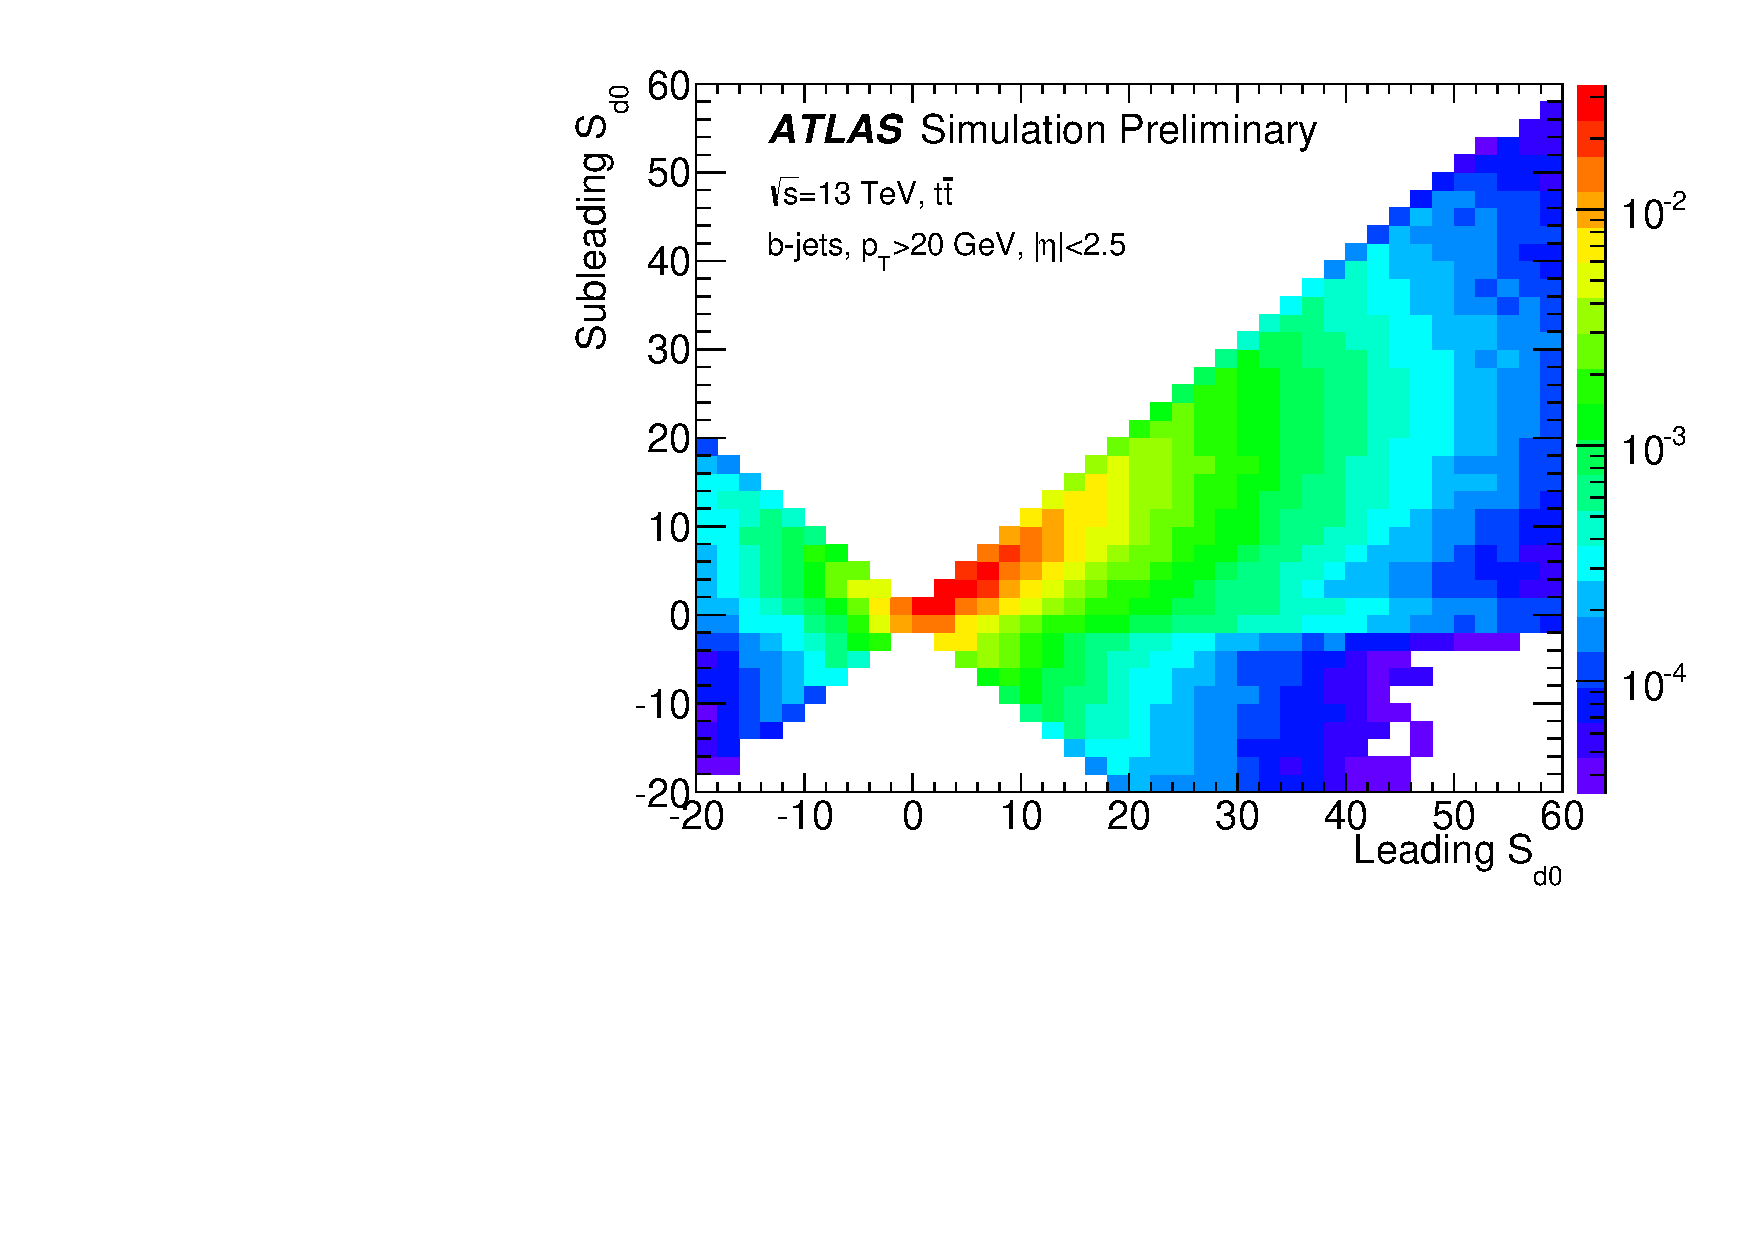
\includegraphics[width=0.48\linewidth]{\figpath/fig_01a}
    } 
     \subfloat[]{ 
            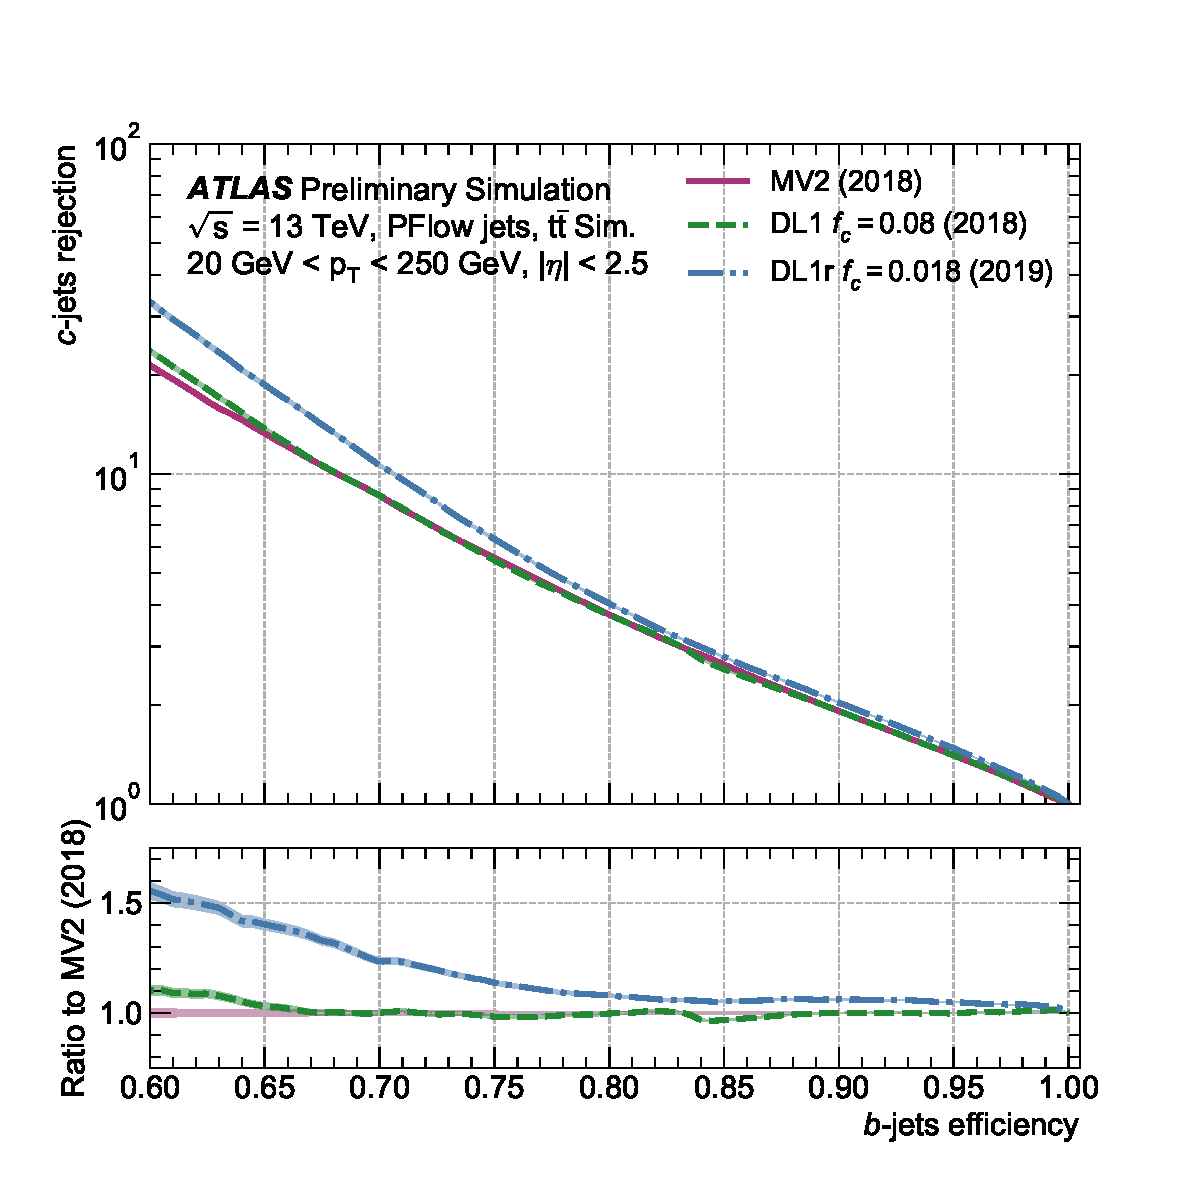
\includegraphics[width=0.48\linewidth]{\figpath/fig_01b}
    } 
    \caption{}
    \label{fig:\jetdef-fig1}
\end{figure}

\begin{figure}[htbp]
    \centering
    % light
    \subfloat[]{ 
            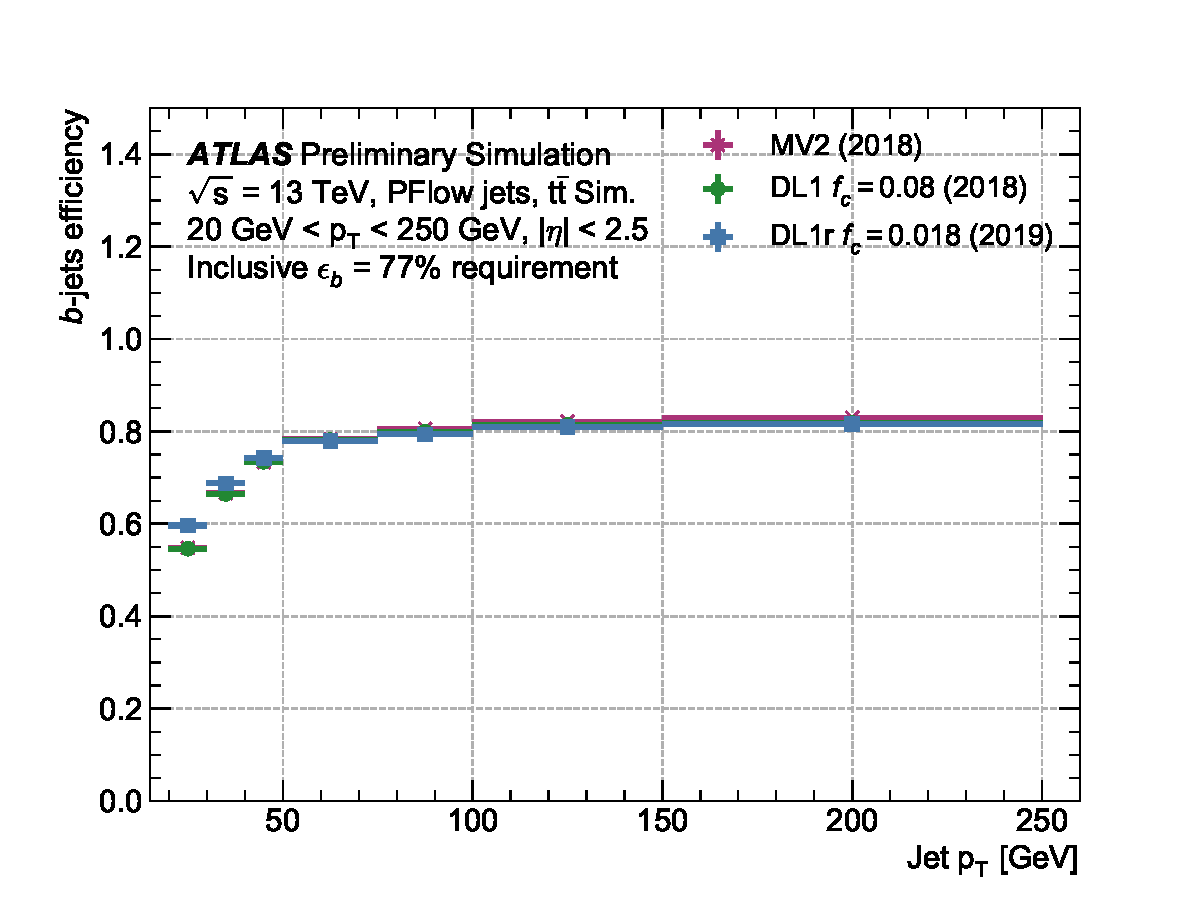
\includegraphics[width=0.33\linewidth]{\figpath/fig_02a}
    } 
     \subfloat[]{ 
            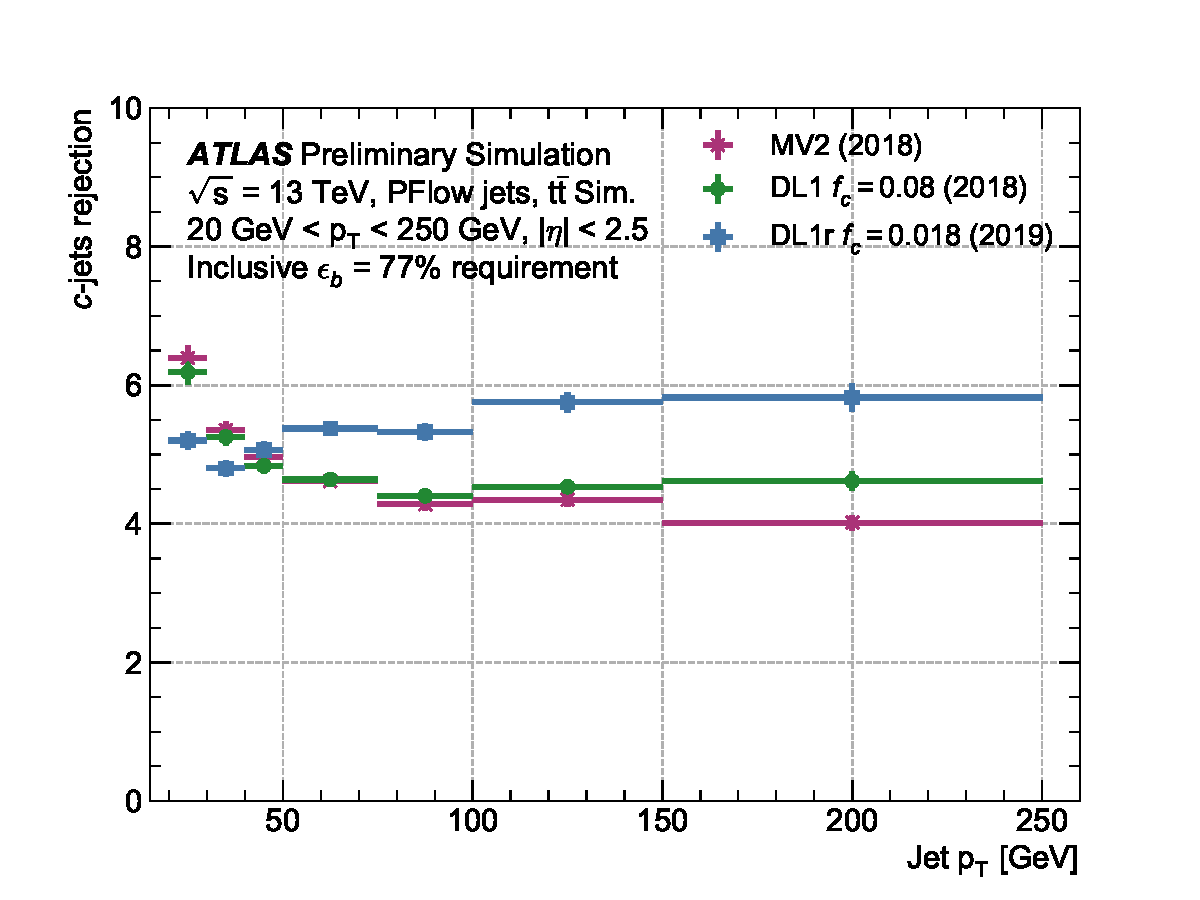
\includegraphics[width=0.33\linewidth]{\figpath/fig_02b}
    } 
    \subfloat[]{ 
            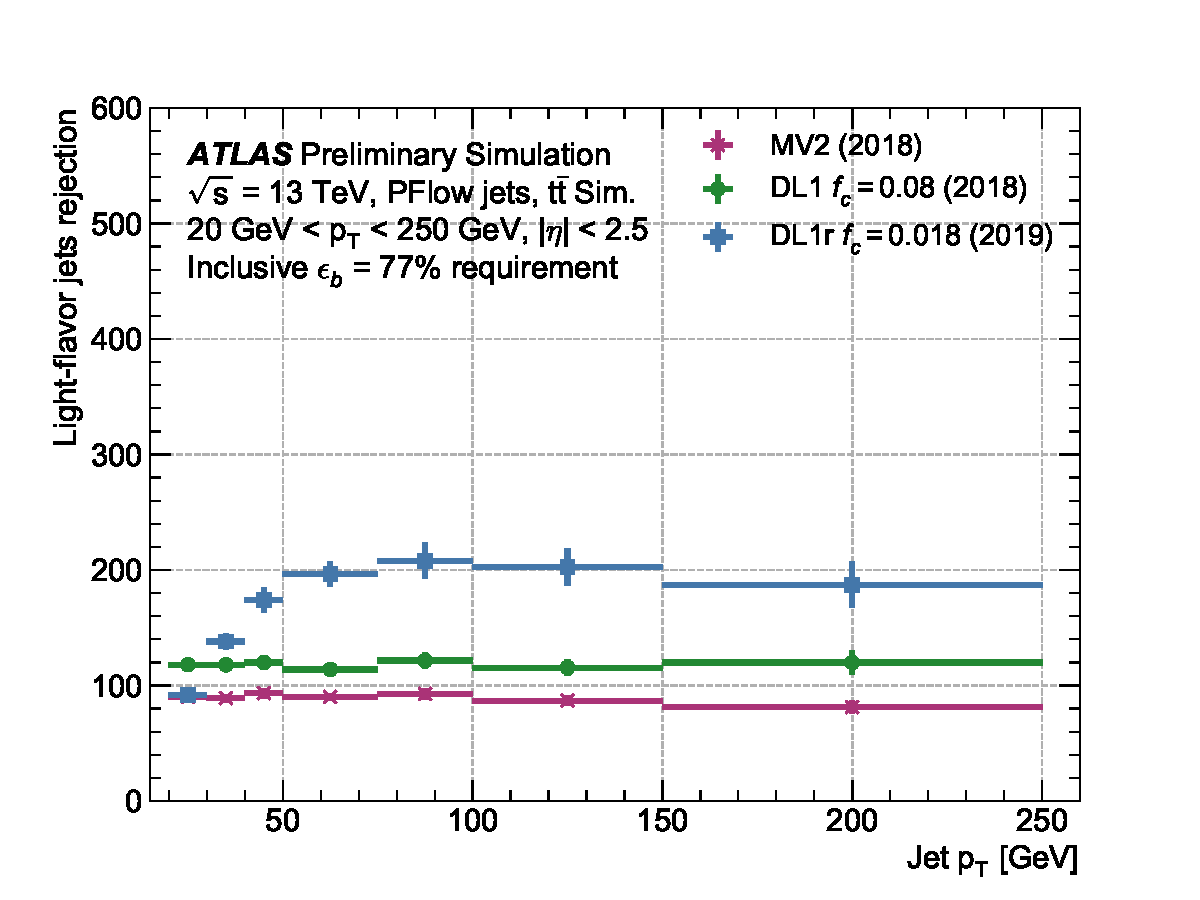
\includegraphics[width=0.33\linewidth]{\figpath/fig_02c}
    } 
    \caption{}
    \label{fig:\jetdef-fig2}
\end{figure}

\begin{figure}[htbp]
    \centering
    % light
    \subfloat[]{ 
            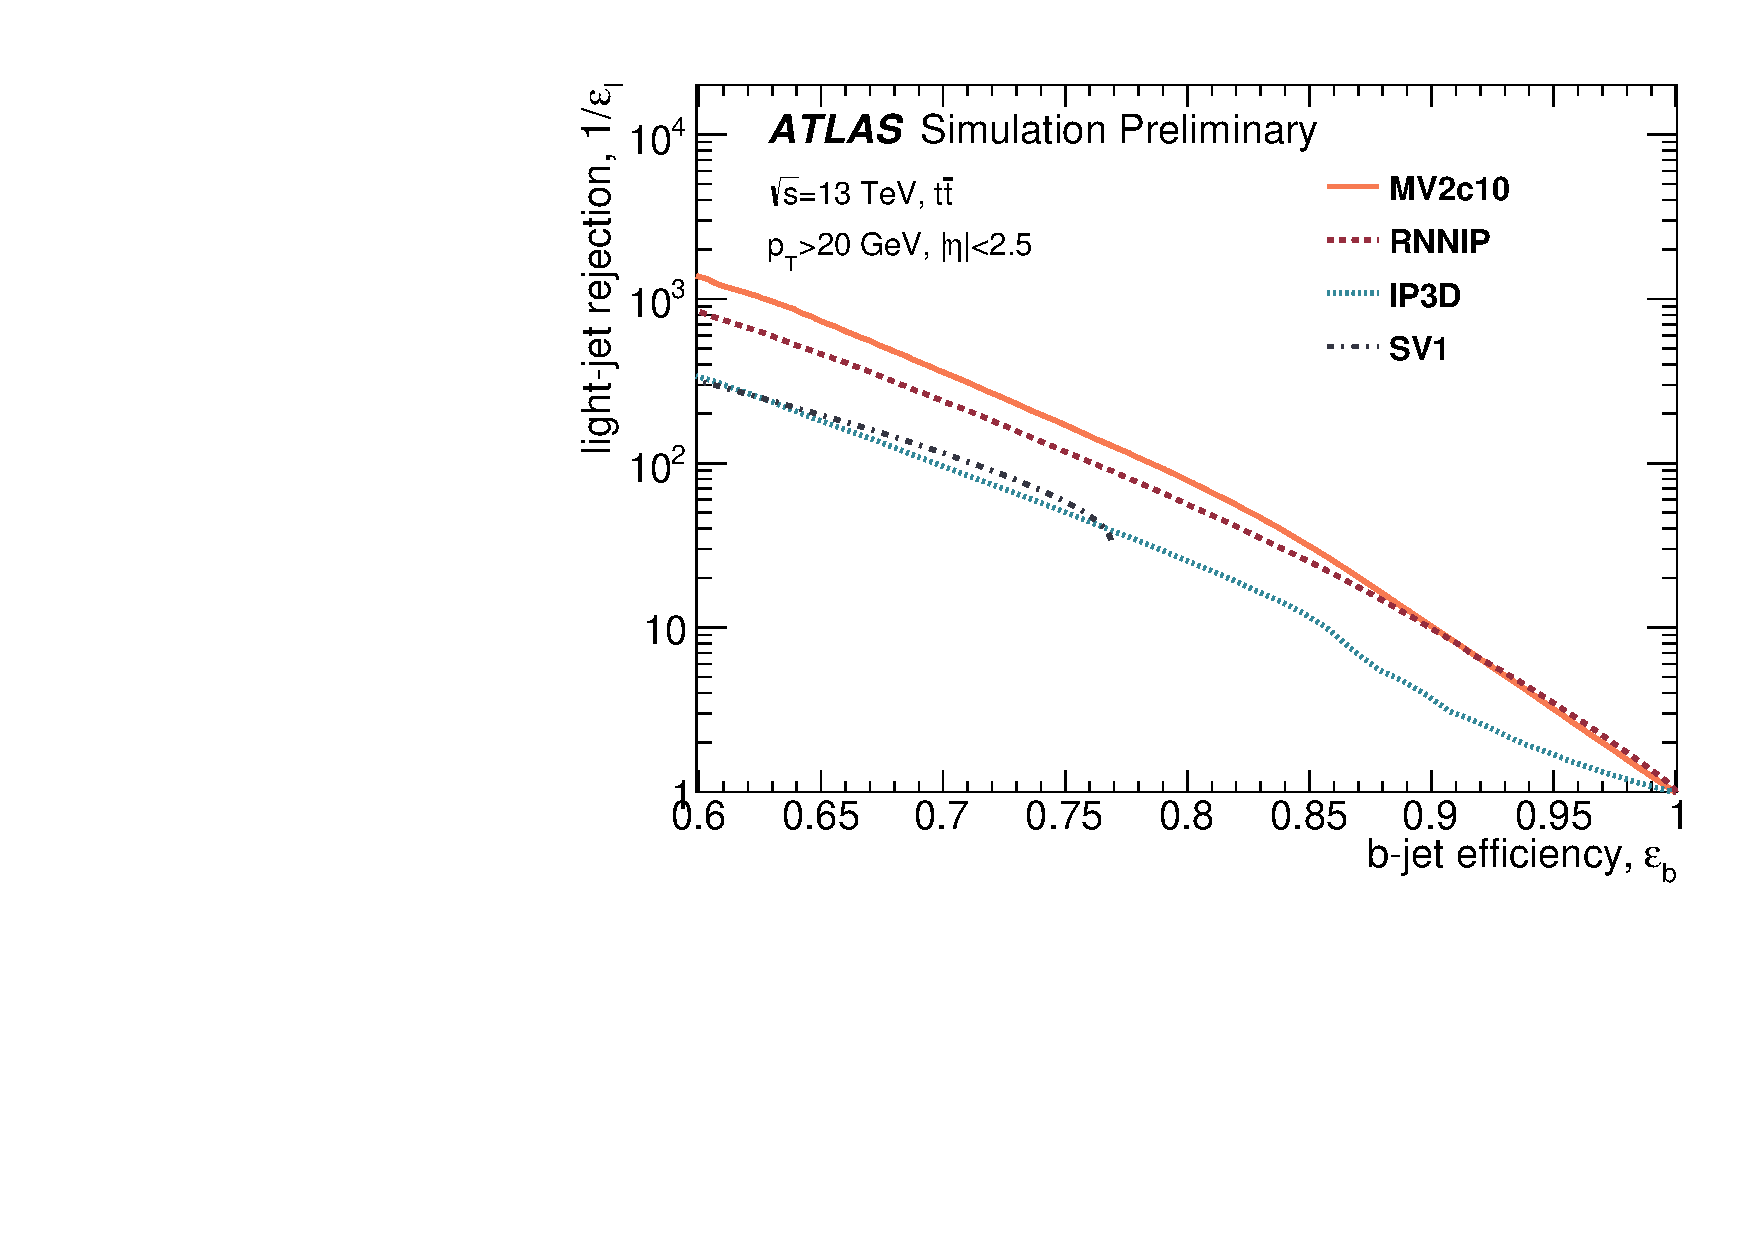
\includegraphics[width=0.48\linewidth]{\figpath/fig_03a}
    } 
     \subfloat[]{ 
            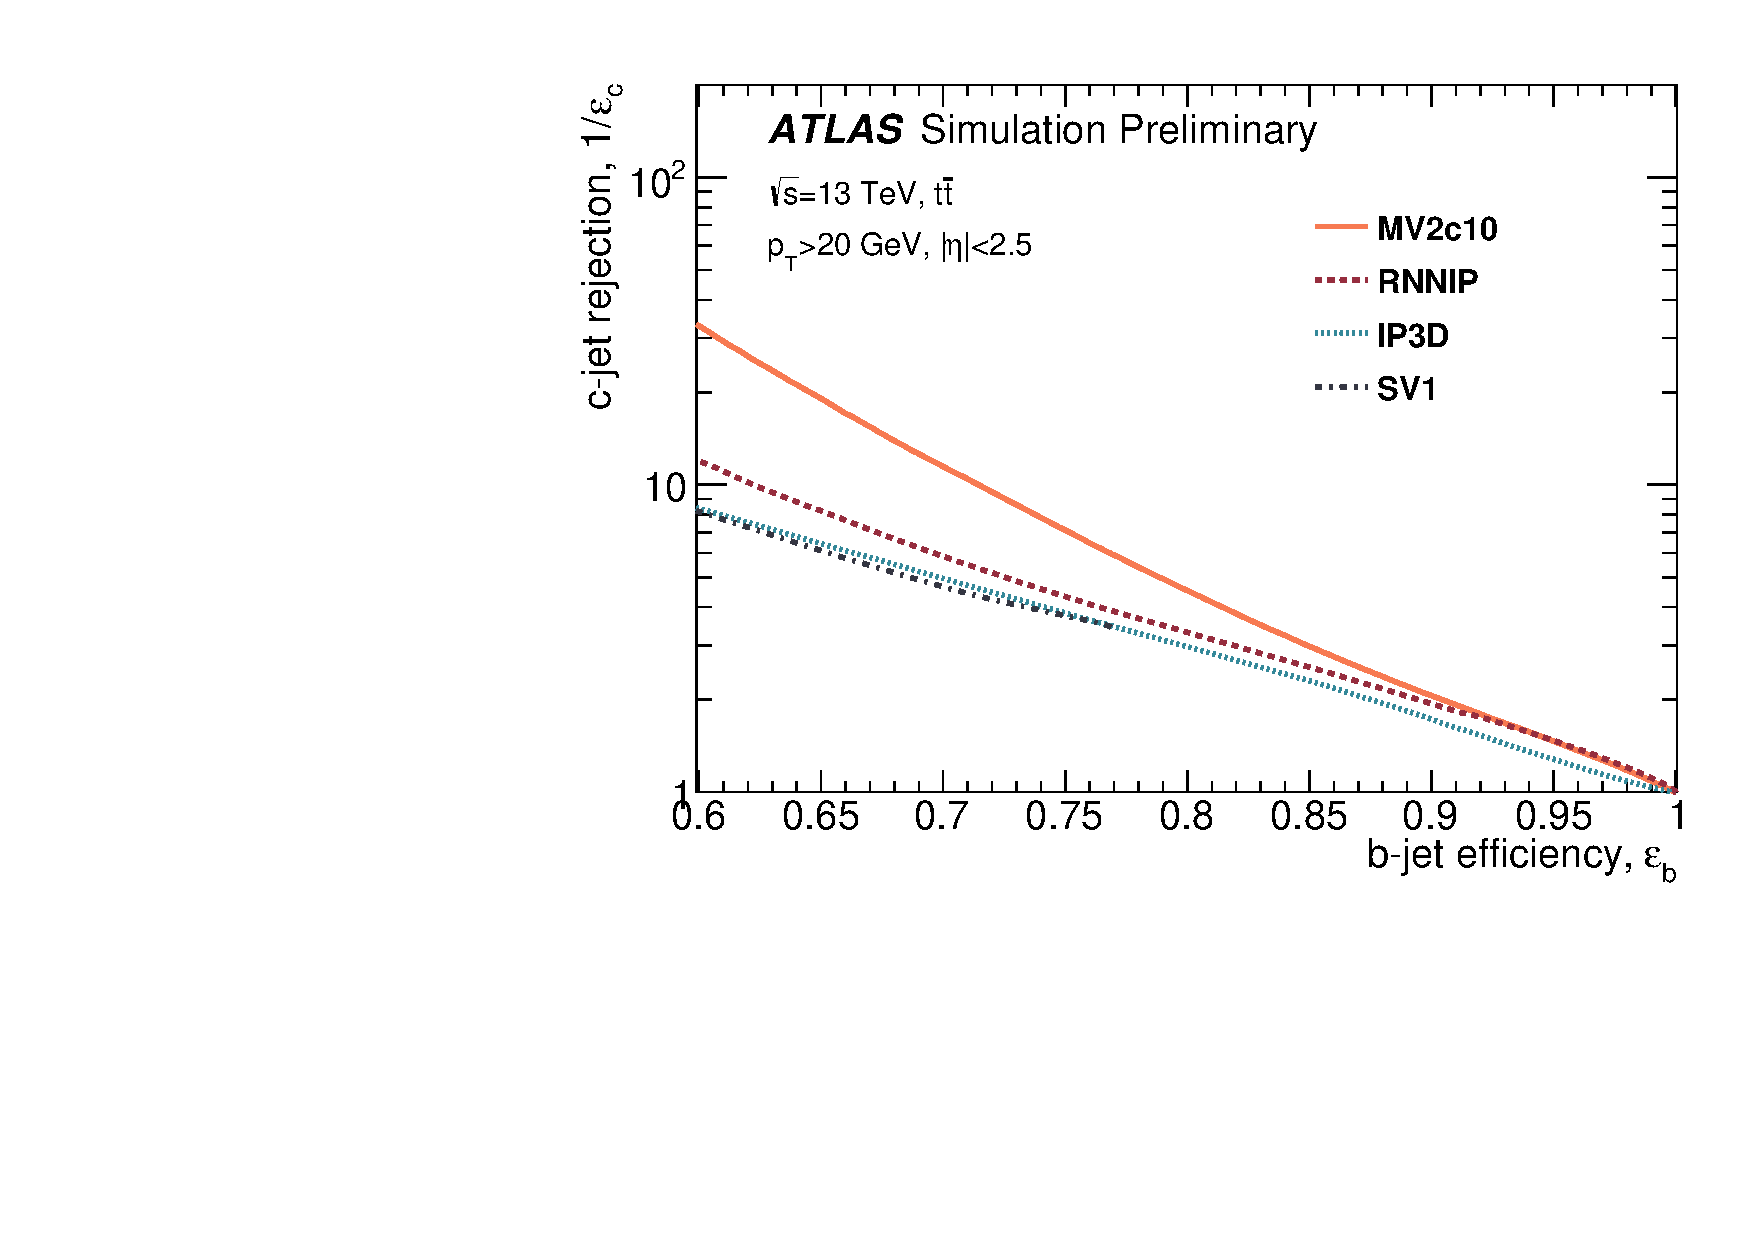
\includegraphics[width=0.48\linewidth]{\figpath/fig_03b}
    } 
    \caption{}
    \label{fig:\jetdef-fig3}
\end{figure}





%%%%%%%%%%%%%%%%%%%%%%%%%%%%%%
% VR track jets
%%%%%%%%%%%%%%%%%%%%%%%%%%%%%%

\FloatBarrier
\clearpage
\subsection{VR track jets optimization}

\hl{I had to have had a dR matching in this plot \ldots let's look up what it was!}

\begin{figure}[htbp]
  \centering
  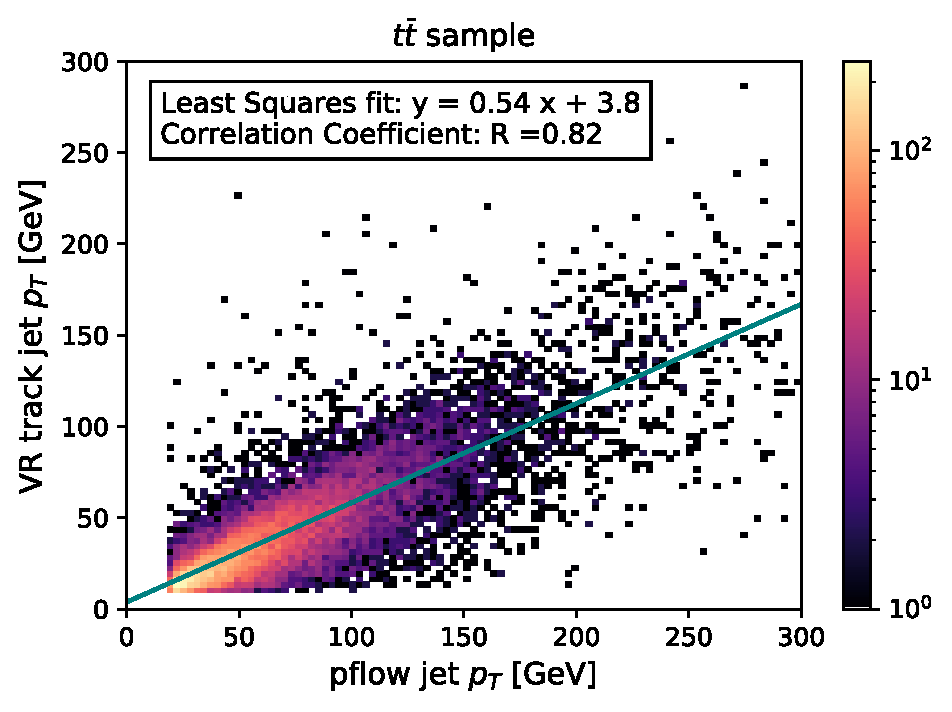
\includegraphics[width=.45\textwidth]{figures/ftag/VR trainings/pt-VR-pflow-ttvar}
  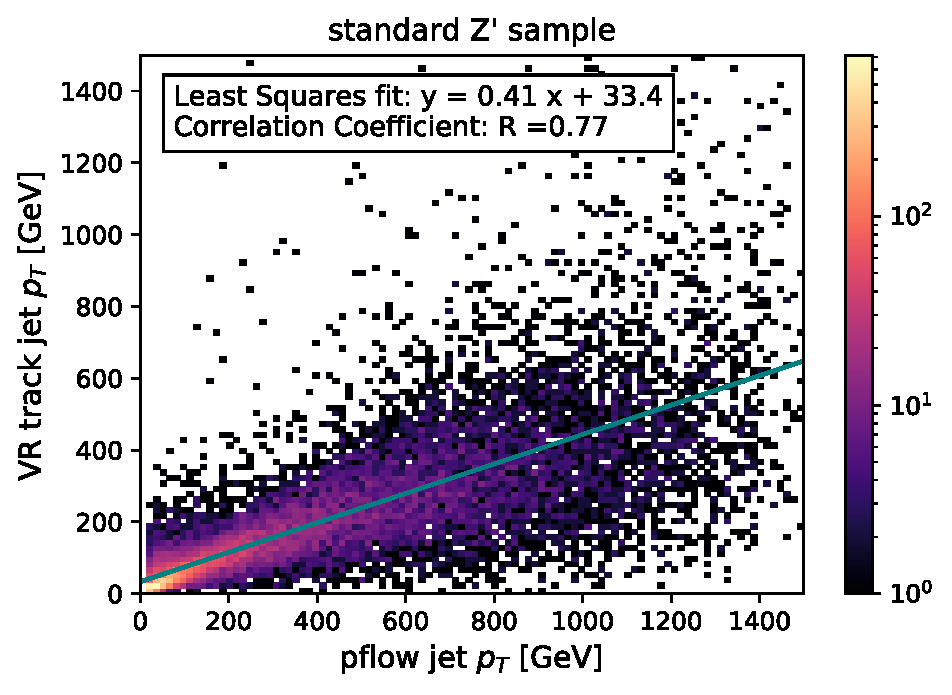
\includegraphics[width=.45\textwidth]{figures/ftag/VR trainings/pt-VR-pflow-std-Zprime}
  \caption{Comparison of the PFlow and VR track jet \pt for jet reconstruction.}
  \label{fig:pt-VR-pflow}
\end{figure}

Note: This plot \emph{motivated} us to move the pT cut on the light and c-jets to 125~GeV (although we kept the b-hadron \pt cut at 250 GeV).

\begin{figure}[htbp]
  \centering
  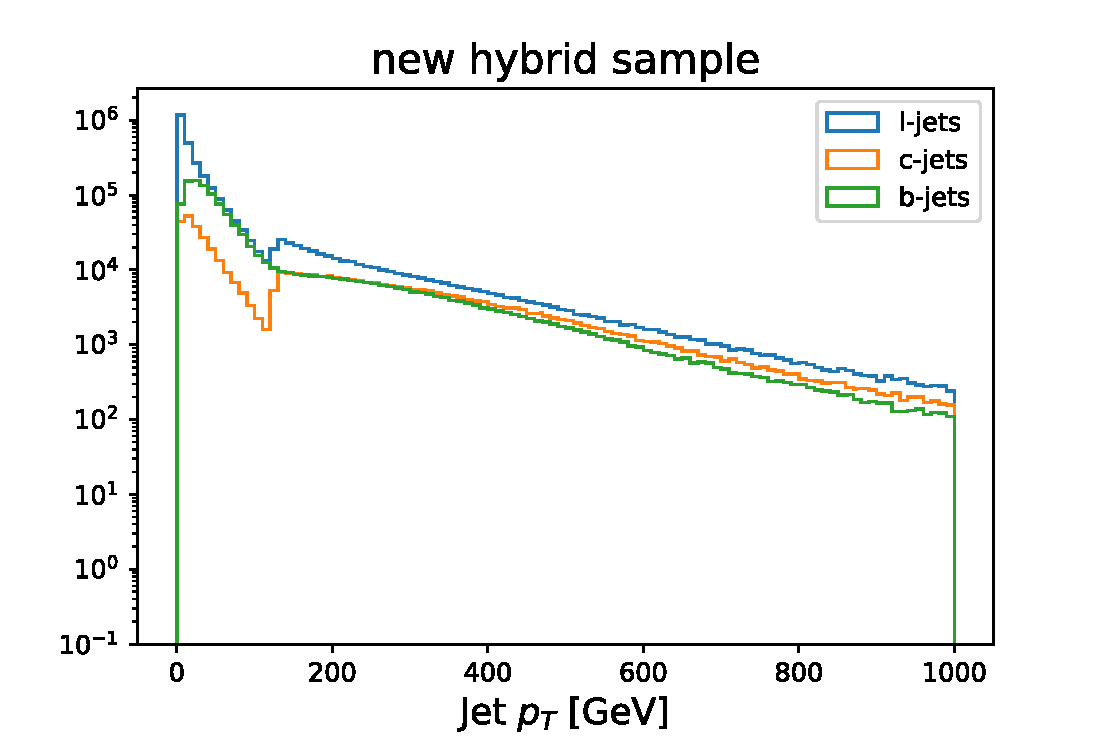
\includegraphics[width=.6\textwidth]{figures/ftag/VR trainings/pt-hyb-vr}
  \caption{The \pt spectrum for the VR track jets using the modified sample cut of 125~GeV for the light jet and \Pqb-jet \pt.}
  \label{fig:pflow-pt-extended-hybrid}
\end{figure}



\begin{figure}
\centering
\subfloat[light rejection]{
	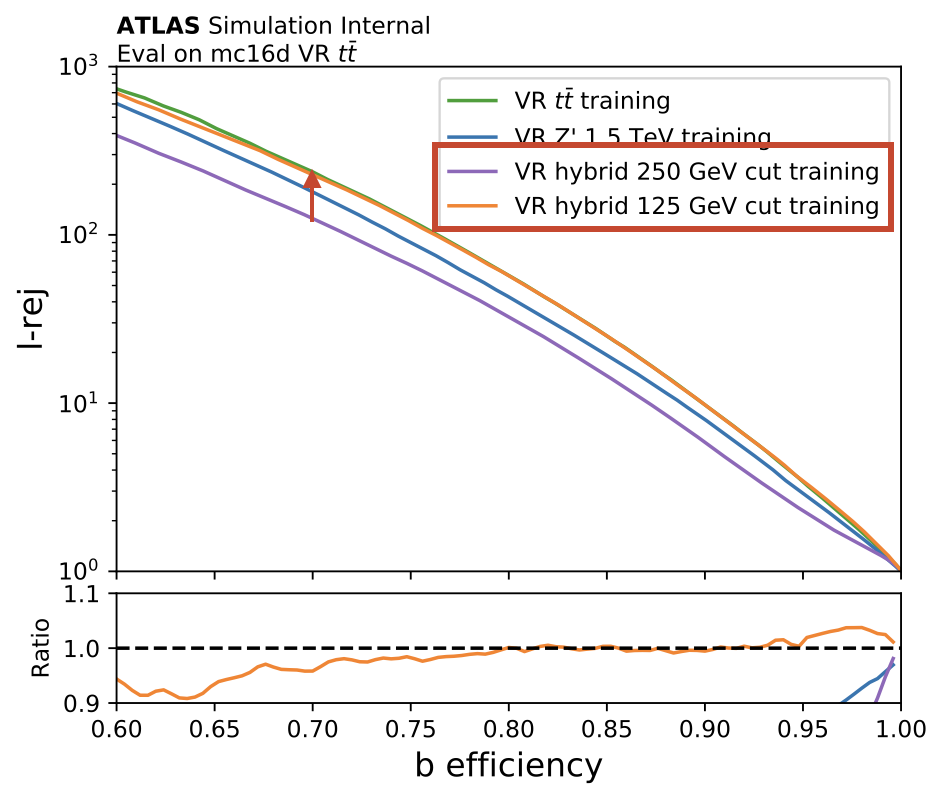
\includegraphics[width=0.45\textwidth]{{figures/ftag/VR\ Trainings/roc-new-cut-l-ttbar}}
	}
\subfloat[\Pqc rejection]{
	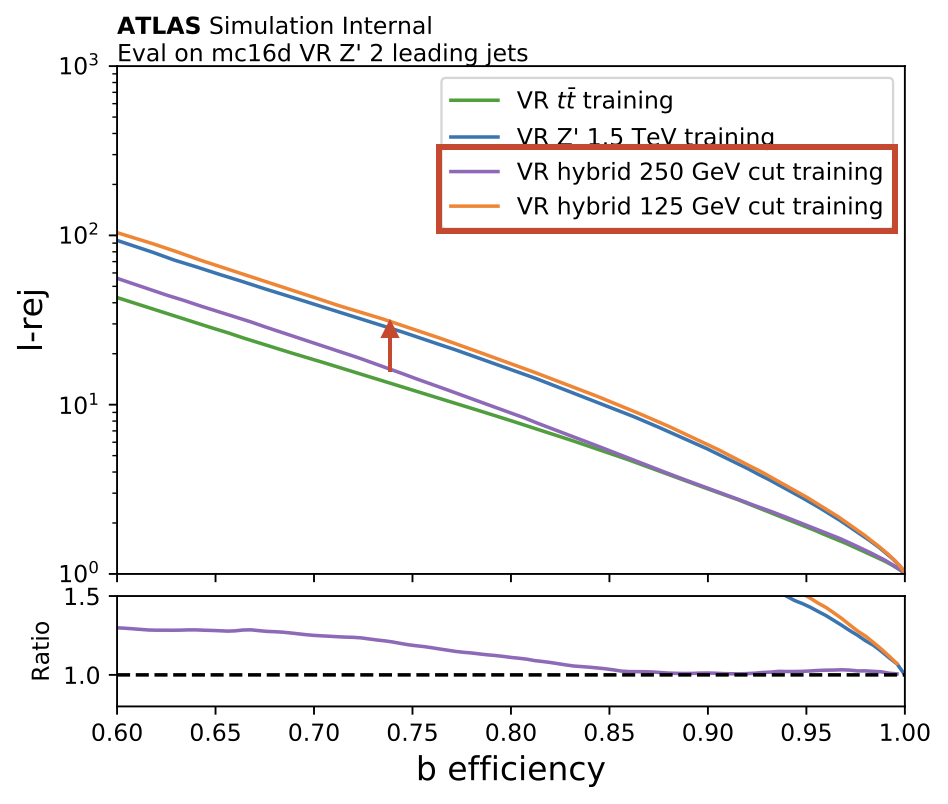
\includegraphics[width=0.45\textwidth]{{figures/ftag/VR\ Trainings/roc-new-cut-l-Zprime}}
	}
\caption{}
\label{fig:VR-improvements}
\end{figure}



\begin{figure}
\centering
\subfloat[light rejection]{
	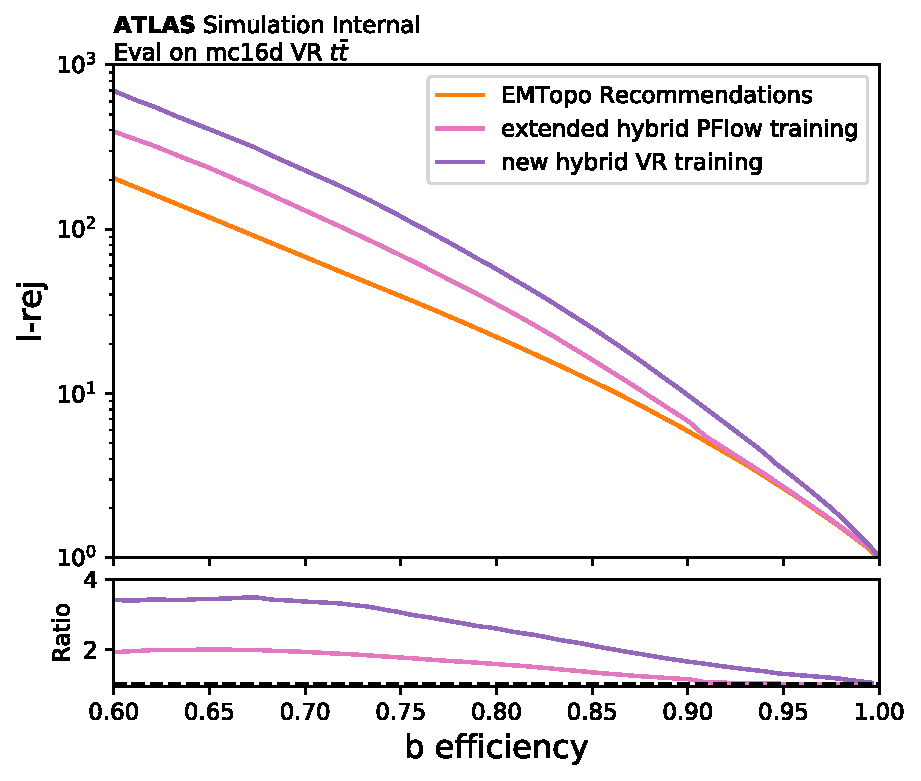
\includegraphics[width=0.45\textwidth]{{figures/ftag/VR\ Trainings/roc-vr-trainings-l}}
	}
\subfloat[\Pqc rejection]{
	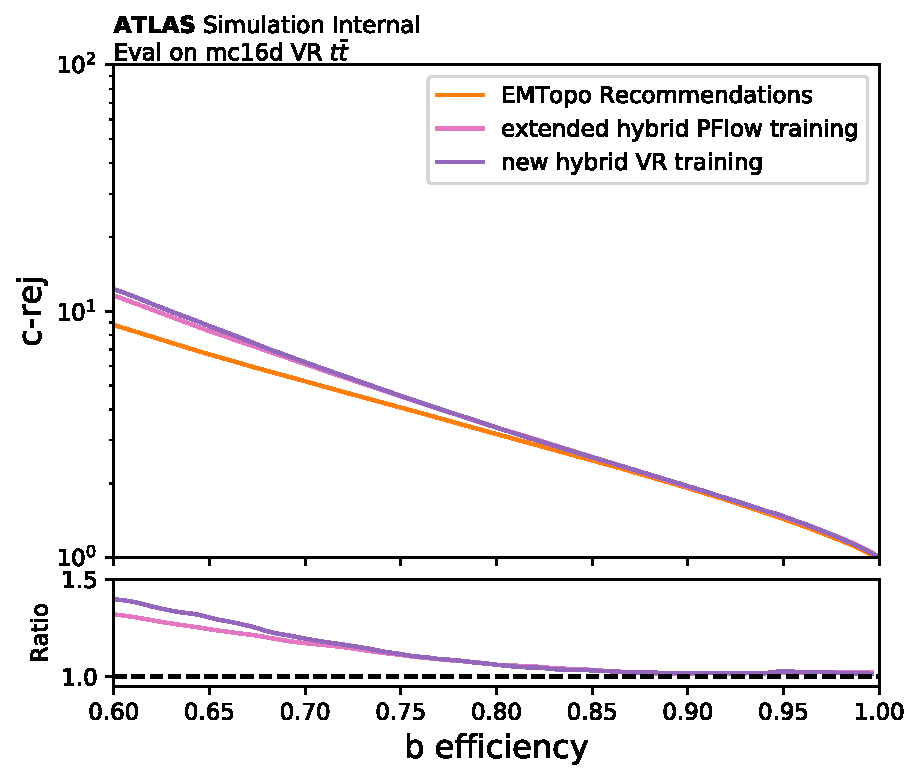
\includegraphics[width=0.45\textwidth]{{figures/ftag/VR\ Trainings/roc-vr-trainings-c}}
	}
\caption{}
\label{fig:VR-improvements}
\end{figure}

\begin{enumerate}
	\item \textcolor{orange}{EMTopo Rec: What we were applying to VR track jets now}
	\item \textcolor{deeppink}{Ext Pflow: If we applied the my new pflow training to VR track jets}
	\item \textcolor{mediumpurple}{New hybrid VR training: NEW dedicated VR training}
\end{enumerate}




\def\jetdef{VR}
% http://atlas.web.cern.ch/Atlas/GROUPS/PHYSICS/PLOTS/FTAG-2019-006/

\def\figpath{figures/ftag/\jetdef \ trainings}

\begin{figure}[htbp]
    \centering
    % light
    \subfloat[]{ 
            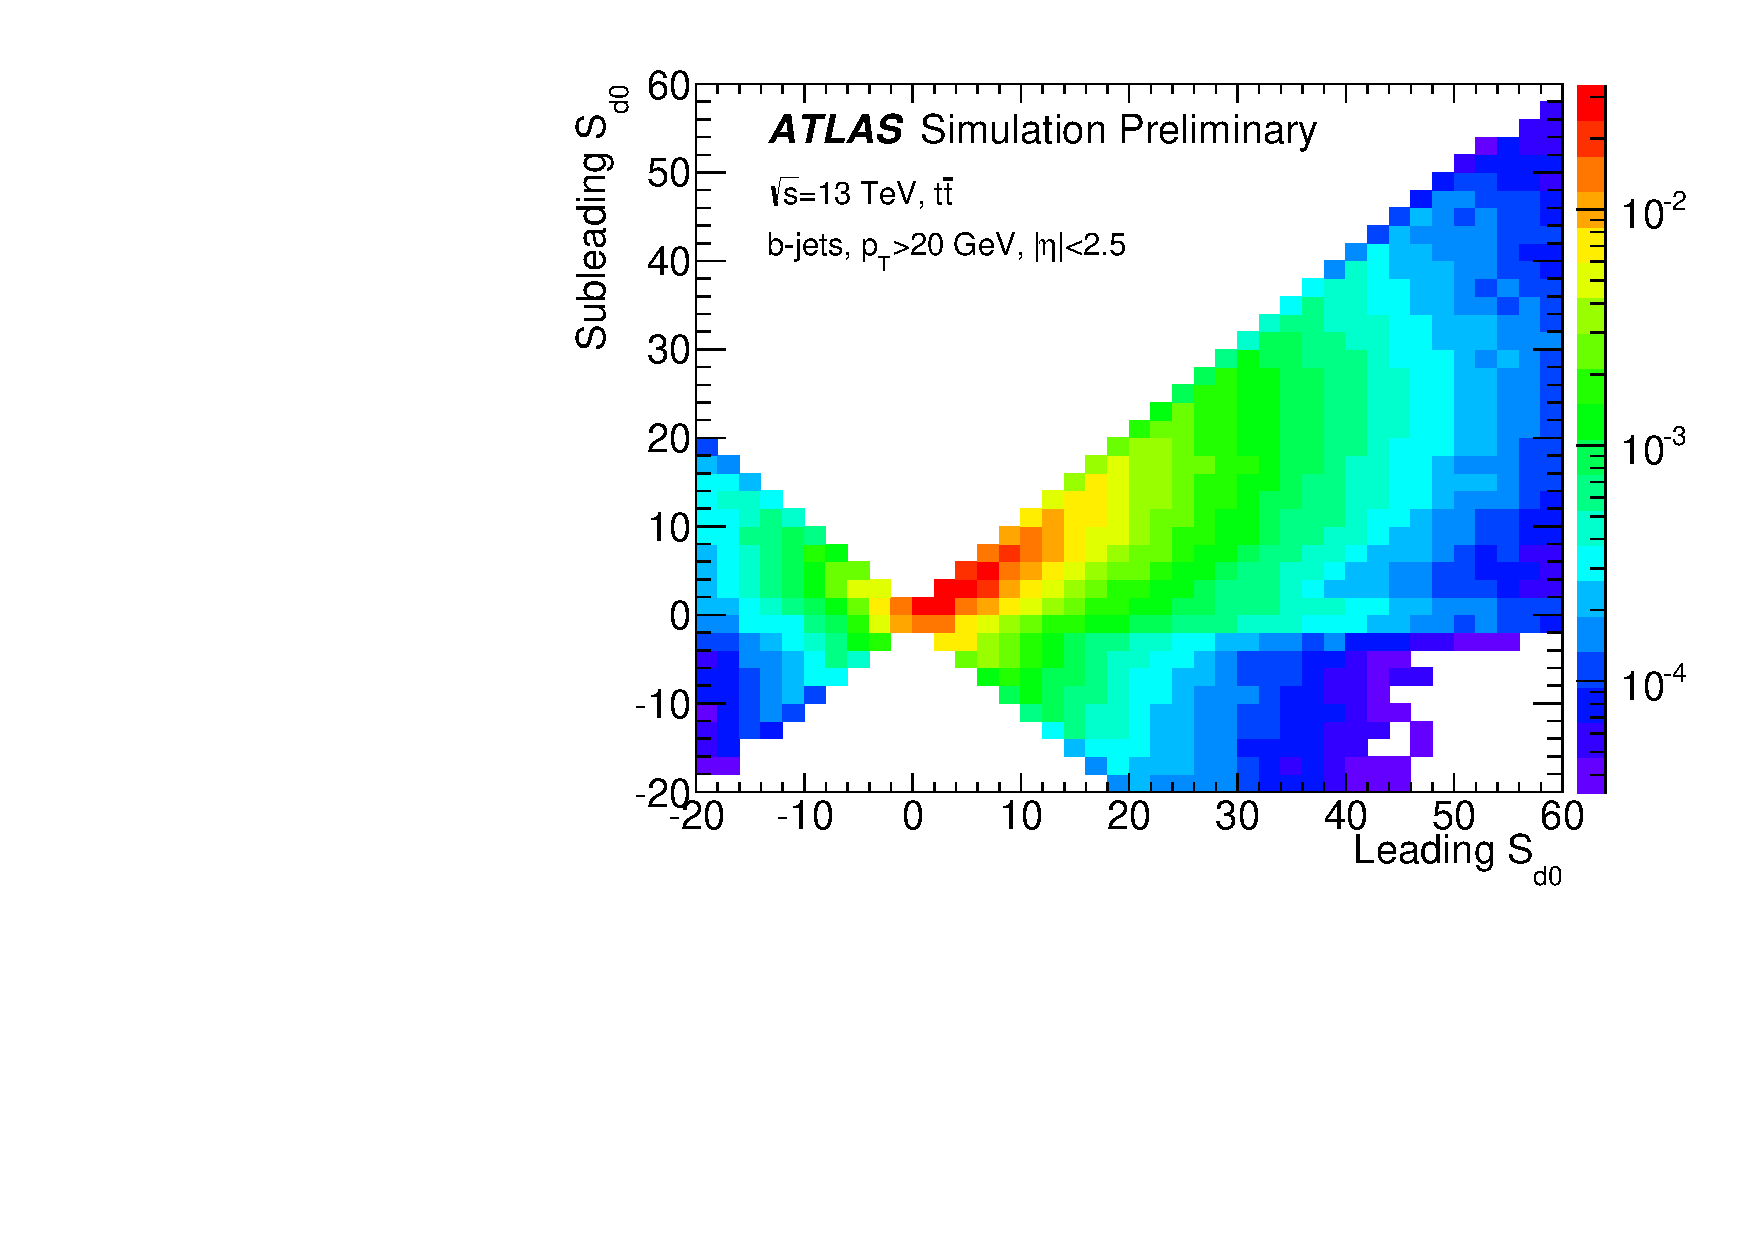
\includegraphics[width=0.48\linewidth]{\figpath/fig_01a}
    } 
     \subfloat[]{ 
            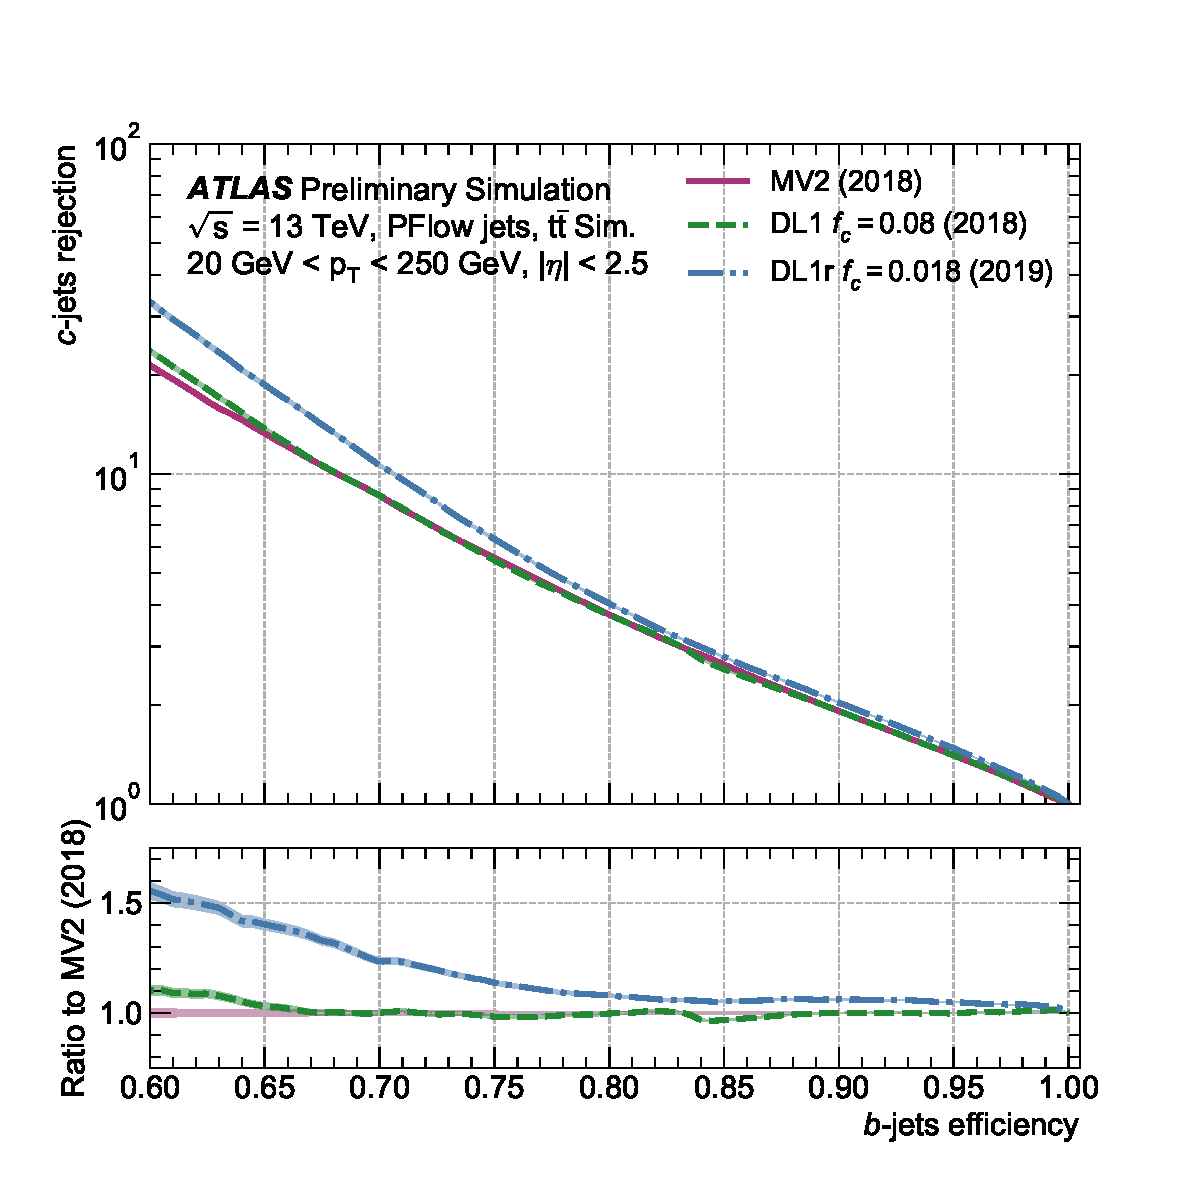
\includegraphics[width=0.48\linewidth]{\figpath/fig_01b}
    } 
    \caption{}
    \label{fig:\jetdef-fig1}
\end{figure}

\begin{figure}[htbp]
    \centering
    % light
    \subfloat[]{ 
            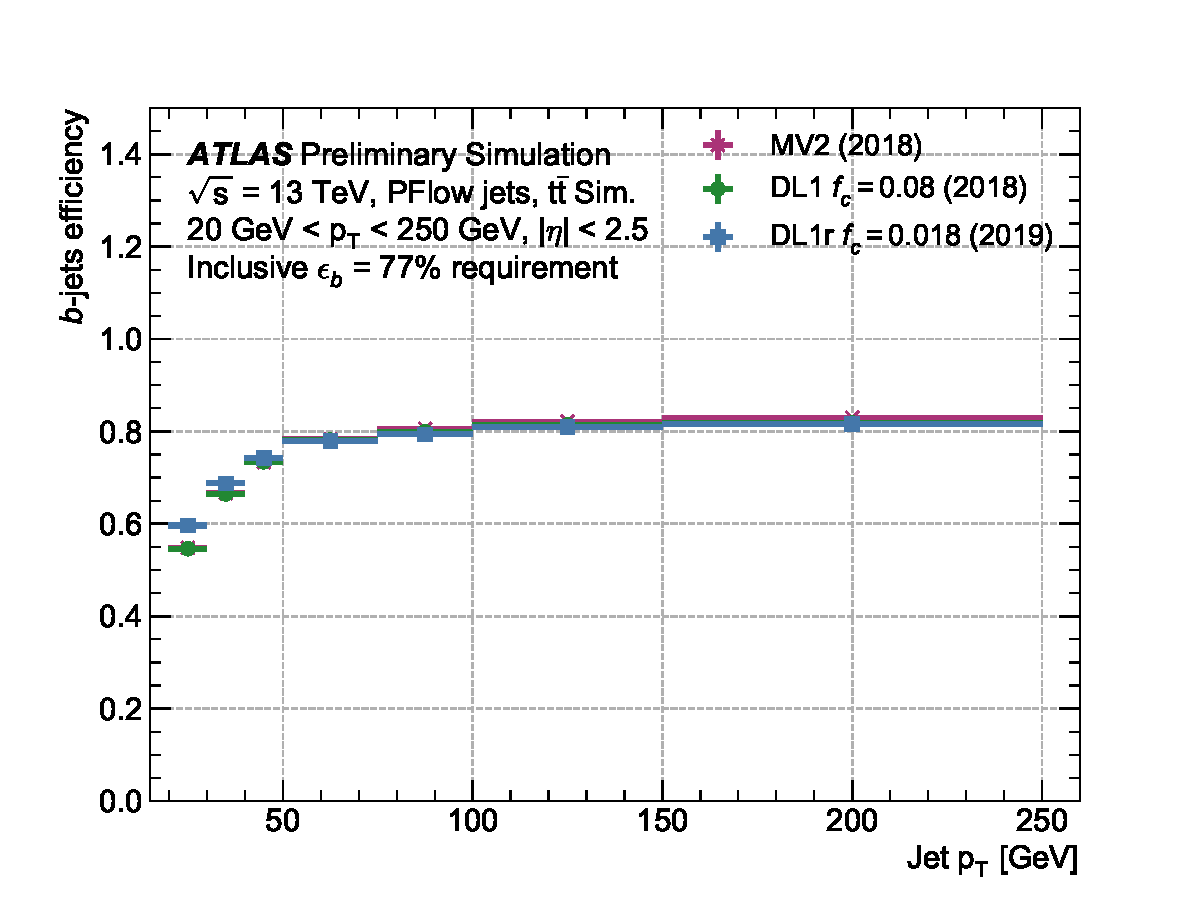
\includegraphics[width=0.33\linewidth]{\figpath/fig_02a}
    } 
     \subfloat[]{ 
            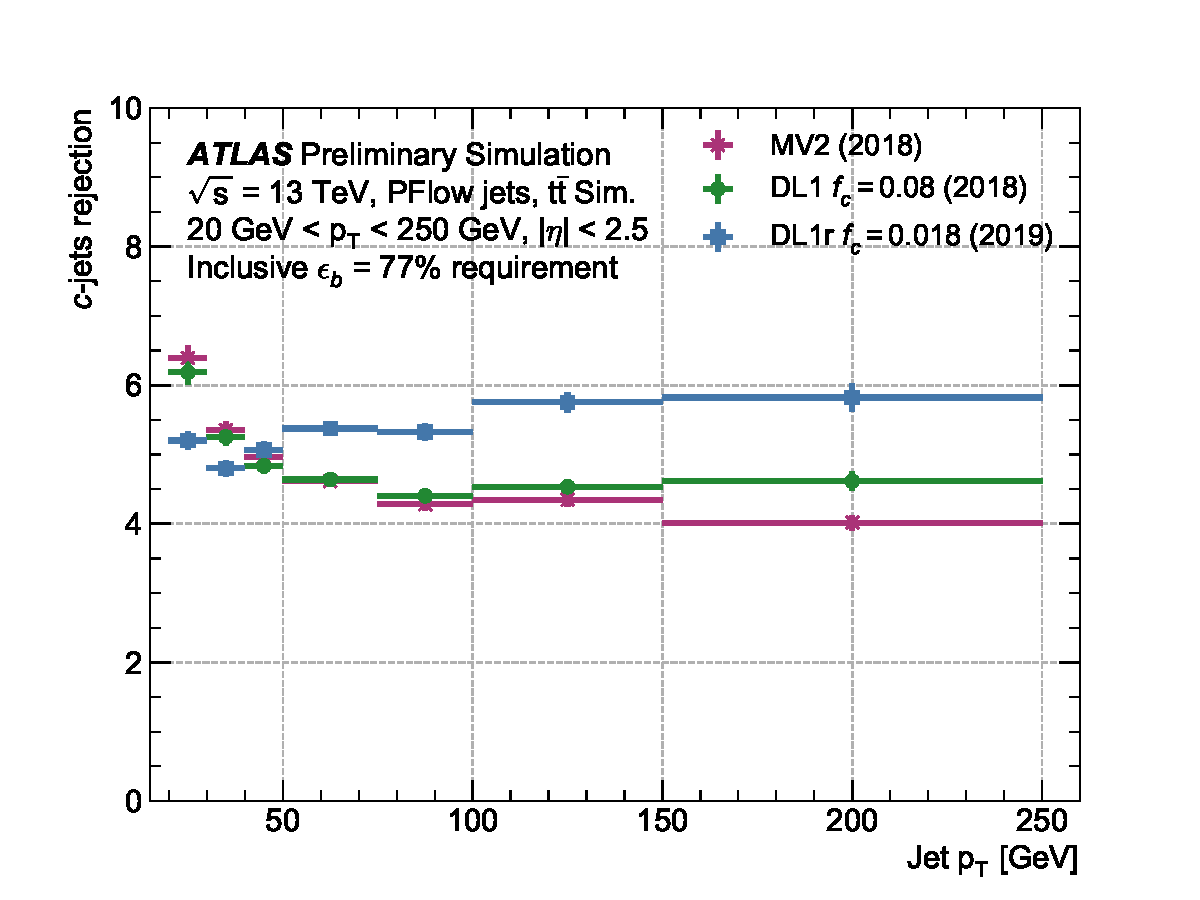
\includegraphics[width=0.33\linewidth]{\figpath/fig_02b}
    } 
    \subfloat[]{ 
            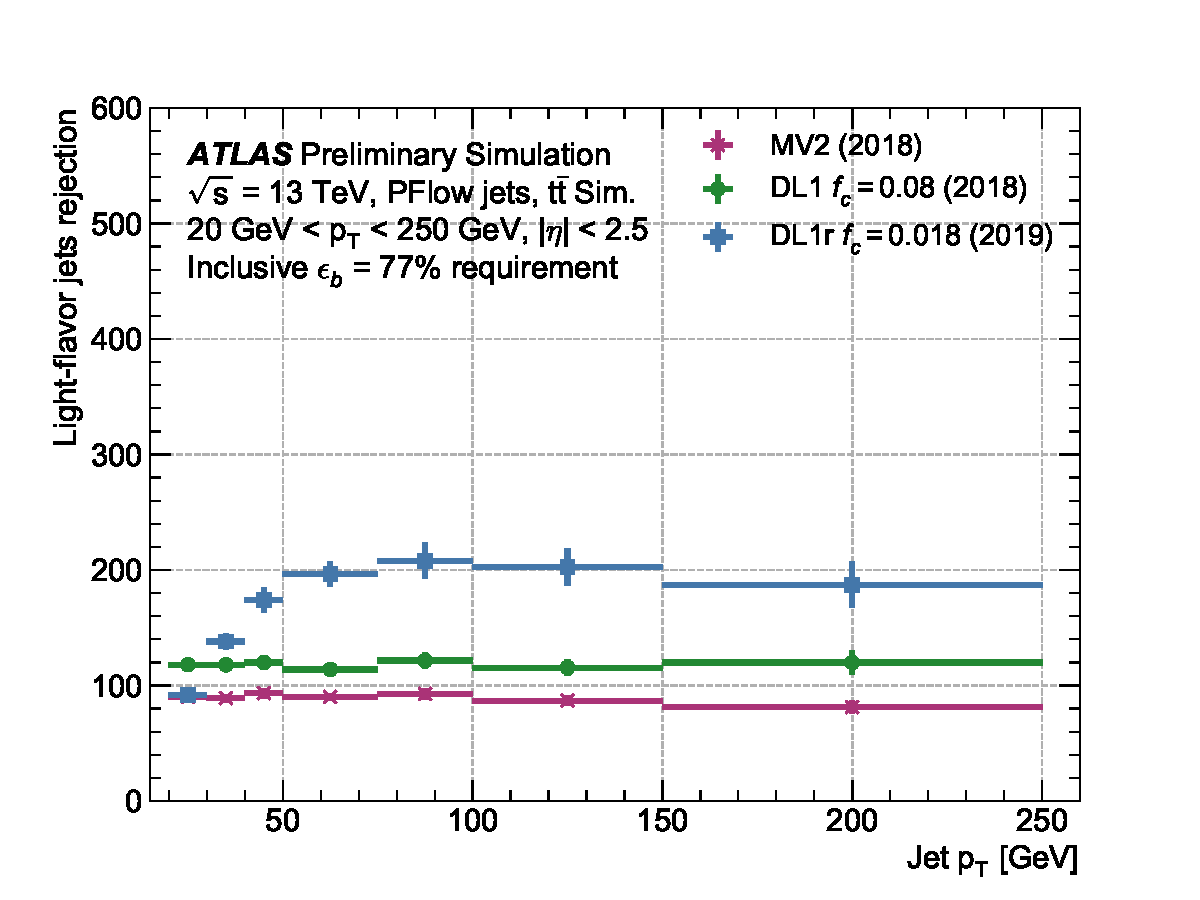
\includegraphics[width=0.33\linewidth]{\figpath/fig_02c}
    } 
    \caption{}
    \label{fig:\jetdef-fig2}
\end{figure}

\begin{figure}[htbp]
    \centering
    % light
    \subfloat[]{ 
            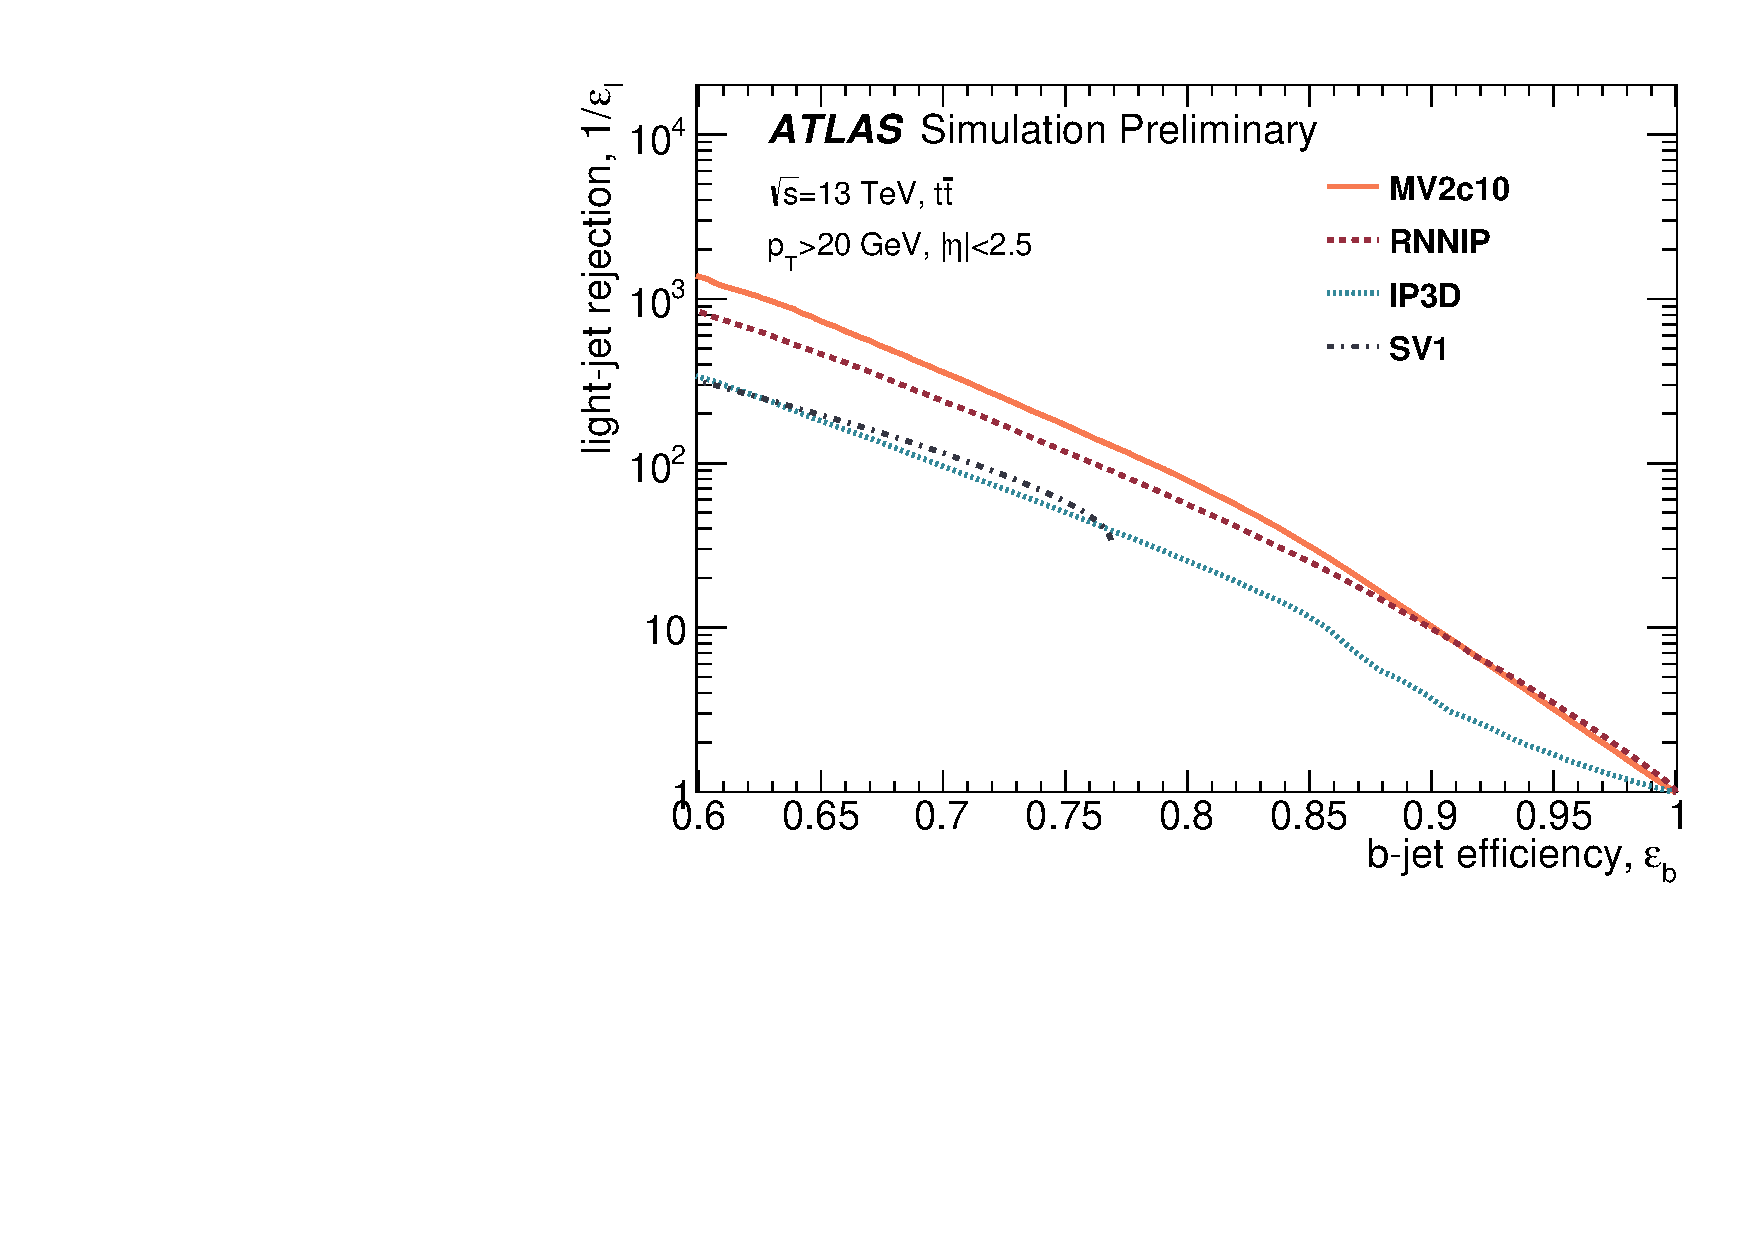
\includegraphics[width=0.48\linewidth]{\figpath/fig_03a}
    } 
     \subfloat[]{ 
            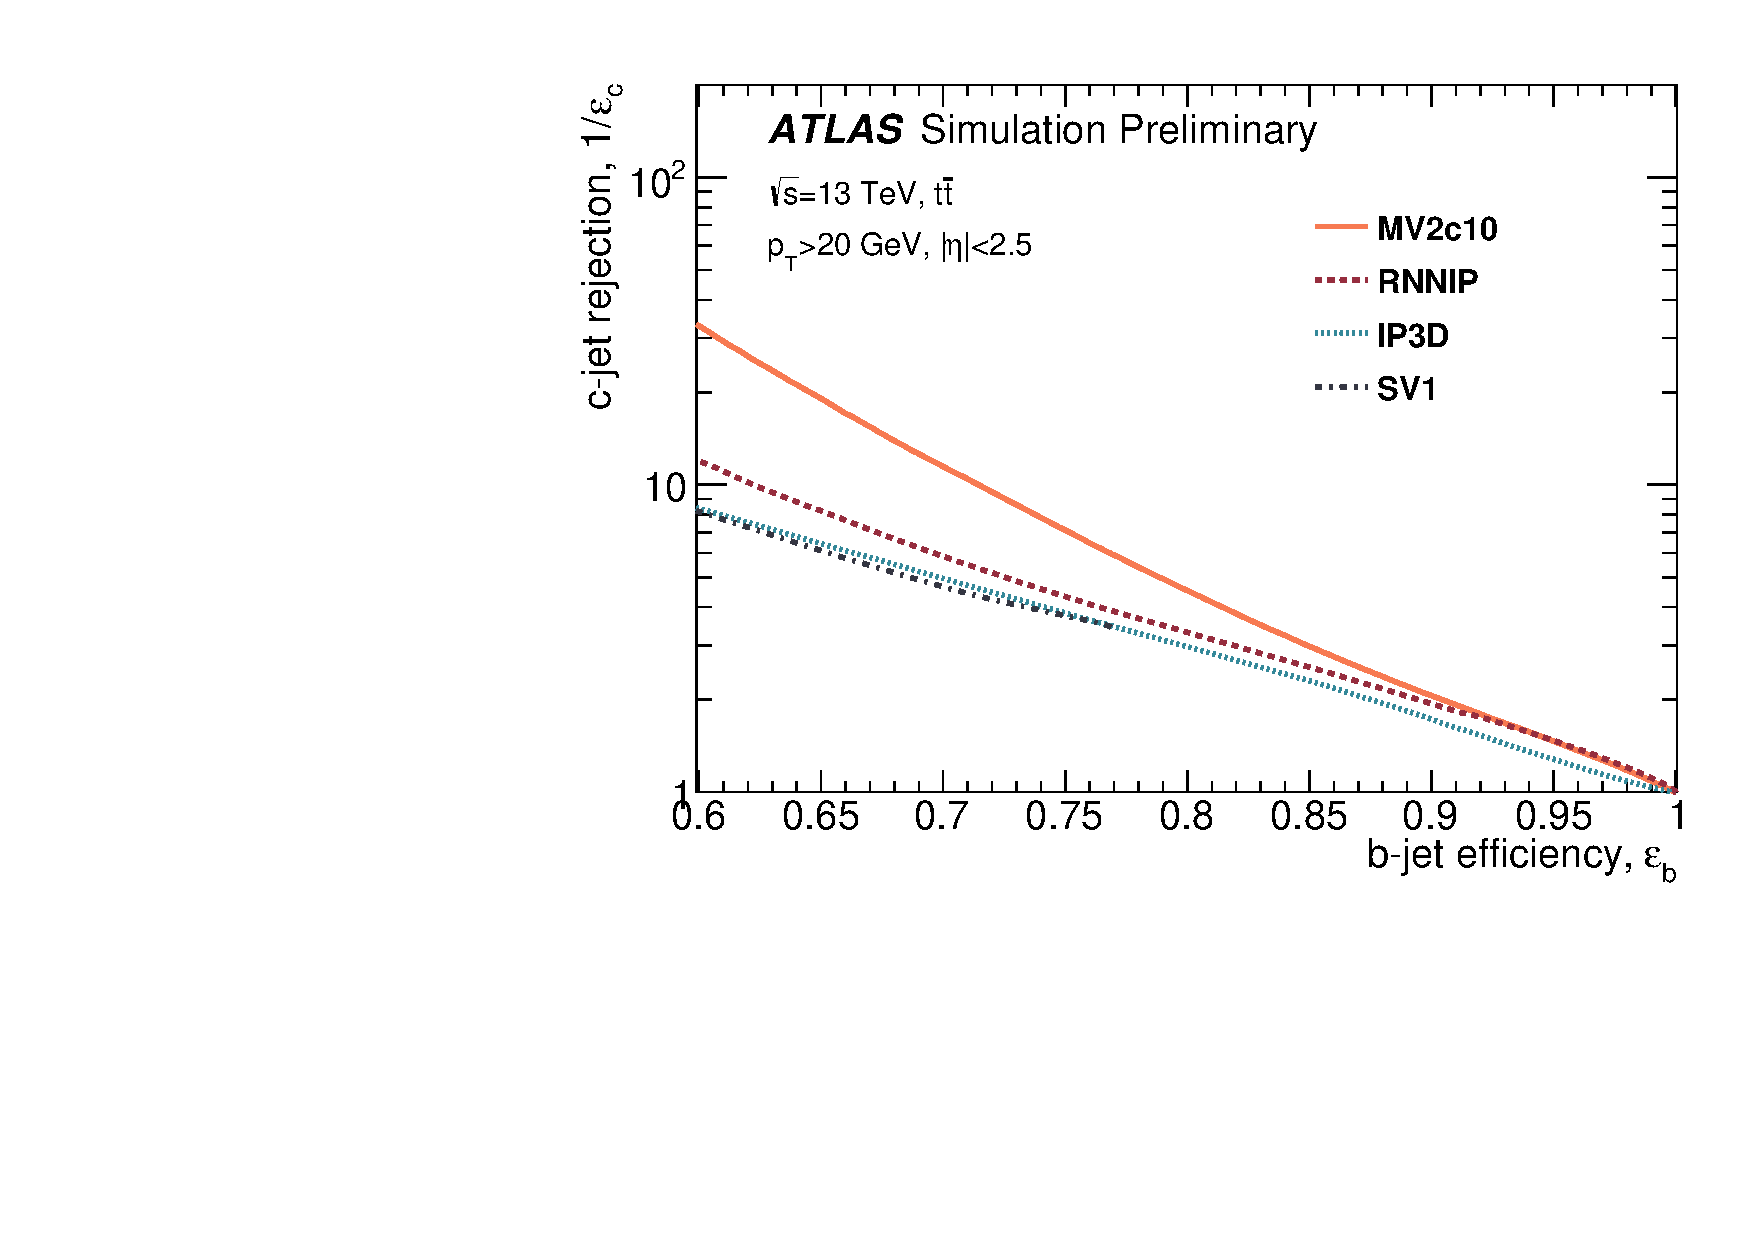
\includegraphics[width=0.48\linewidth]{\figpath/fig_03b}
    } 
    \caption{}
    \label{fig:\jetdef-fig3}
\end{figure}

\subsection{Impact of FTAG improvements on analyses}

\begin{figure}
\centering
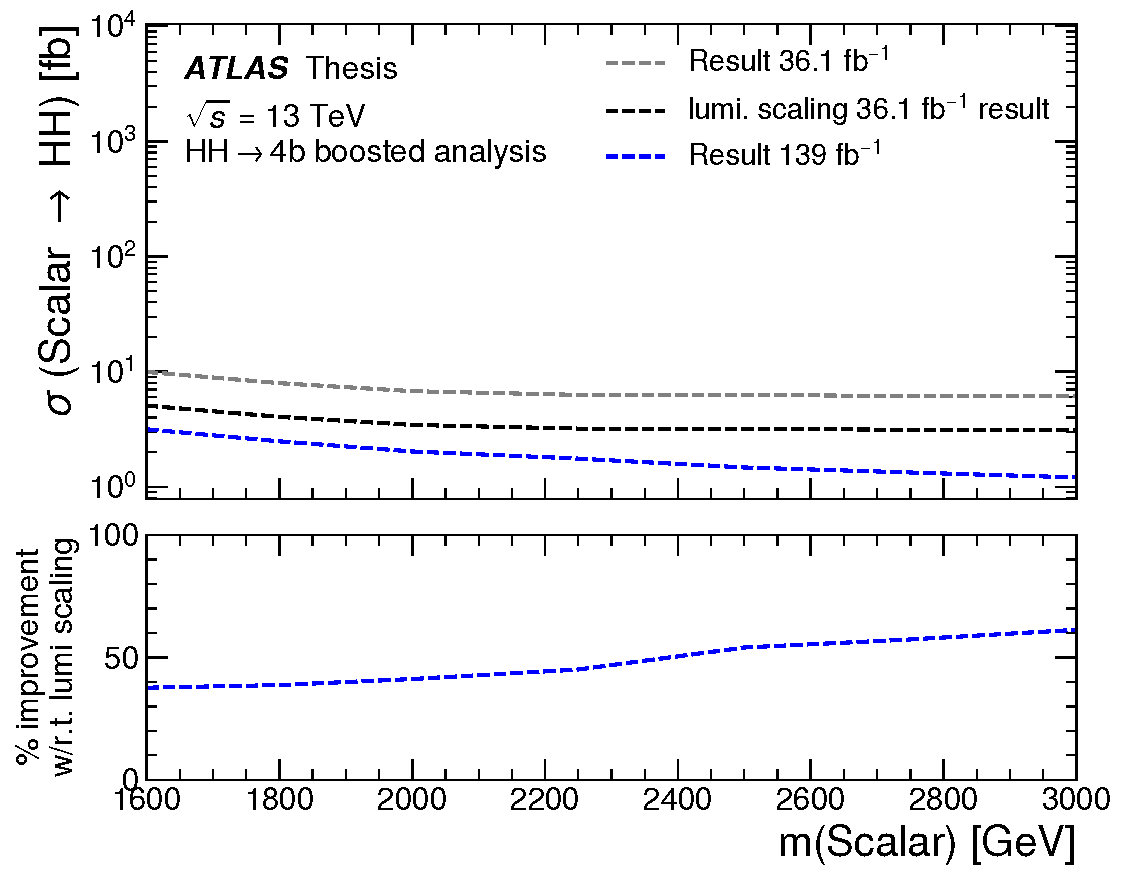
\includegraphics[width=\textwidth]{figures/my_dihiggs/HH4b-boosted-vr-trk-jet-improvements.pdf}
\caption{Need to cite the 36 ifb and 139 ifb.}
\label{fig:boosted-vr-trk-jet-improvements}
\end{figure}
